



%--------------------------------------


\newpage

%\section[Network Growth Models][Modèles de Croissance de Réseau]{Network Growth Models : Explicative power for various approaches}{Modèles de Croissance de Réseau}
\section{Network Growth Models}{Modèles de Croissance de Réseau}


\label{sec:networkgrowth}


%--------------------------------------

Nous proposons dans un premier temps d'étudier en détails les processus de croissance de réseau pour l'échelle mesoscopique. L'idée est de comprendre les propriétés intrinsèques des différentes heuristiques de croissance de réseau. Cet exercice est d'une part intéressant en lui-meme puisqu'il n'existe pas a notre connaissance de comparaison systématique de modèles de morphogenèse des réseaux spatiaux : si~\cite{xie2009modeling} propose par exemple une revue du point de vue de l'économie des réseaux, celle-ci ne prend pas en compte certaines disciplines d'une part (voir Chapitre~\ref{ch:modelinginteractions}), et ne compare pas les performances des modèles par des implémentations dédiées comparables. 


%--------------------------------------

%%%%%%%%%%%%%%%%%%%%
\subsection{Benchmarking Network growth heuristics}{Comparer les heuristiques de croissance de réseau}


\bpar{
Considering Network Growth in itself, many heuristics are available to generate a network under some constraints. As already developed, from economic network growth approach to local optimization heuristics, geographical mechanisms or biological network growth, each has its advantages and particularities.
}{
Pour la croissance du réseau en tant que telle, de nombreuses heuristiques existent pour générer un réseaux sous certaines contraintes. Comme déjà développé précédemment notamment en~\ref{sec:modelingsa}, des modèles économiques de croissance de réseau au heuristiques d'optimisation locale, aux mécanismes géographiques ou à la croissance de réseau biologique, chacun a ses avantages et particularités propres. Nous avons déjà testé en~\ref{sec:correlatedsyntheticdata} une heuristique basée sur la rupture de potentiel d'interaction. Pour pouvoir comparer ``toutes choses égales par ailleurs'' les différentes heuristiques de génération de réseau, il est nécessaire des les explorer à densité fixée, même si le sens thématique des résultats ne peut avoir de valeur ni sur le temps long, ni pour la co-évolution.
}


L'importance d'heuristiques pouvant capturer une structure topologique permettant un certain compromis entre performance, congestion et coût, est montrée par des analyses empiriques comme \cite{2012arXiv1202.1747W} pour les réseaux de métro, qui montre que les motifs d'évolution des corrélations entre degrés témoignent d'une évolution des réseaux vers une telle topologie.


Nous précisons par la suite le coeur du modèle de croissance de réseau ainsi qu'un certain nombre d'heuristiques aux origines variées, comparées dans des conditions similaires par leur intégration à une base commune.


%%%%%%%%%%%%%%%%%%%%%%%
\subsubsection{Network growth model core}{Base du modèle de croissance de réseau}


Un processus commun aux différentes heuristiques constitue le coeur du modele de croissance de réseau, et fait le pont entre la distribution de densité de population et le réseau. Concrètement, il s'agit d'attribuer des nouveaux centres en fonction de cette densité, et nous faisons le choix de specifier ce processus de manière exogène à la croissance de réseau elle-même\footnote{Cette étape intermédiaire se rapproche dans notre cas d'un esprit de modélisation procédurale, puisque la règle implémentée cherche a reproduire une forme sans besoin des processus reels. Cela pose la question de l'équifinalité et de l'existence potentielle de modèles equivalents pour ce sous-modele ou pour le modele complet capturant un processus reel correspondant a celle-ci. L'utilisation de multi-modélisation également sur cette étape pourrait être une solution mais les cadres permettant de s'extraire d'un nombre arbitraire de niveaux de stationnarité ou même permettant une autonomie du modèle sur ces choix n'existent pas encore.}.


Reprenons le contexte utilisé en~\ref{sec:correlatedsyntheticdata}, c'est à dire une grille de cellules caractérisées par leur population $P_i$, sur laquelle un réseau composé de noeuds et de liens se développe. La distribution de la population sera ici fixe dans le temps $P_i(t) = P_i(0)$, et le réseau évolue séquentiellement à partir d'un réseau initial.

Une étape de croissance de réseau est réalisée à intervalles de temps $t_N$ (paramètre permettant d'ajuster les vitesses respectives d'évolution pour la population et pour le réseau). Elle correspond aux étapes suivantes, dont les deux premières raffinent la logique de~\cite{raimbault2014hybrid} (qui stipule que des centres de peuplement doivent être connectés au réseau existant de manière basique) :

\begin{enumerate}
	\item Un nombre fixe $n_N$ de nouveaux noeuds est ajouté. Séquentiellement, la probabilité de recevoir un nouveau noeud est donnée par
\[
p_i = \frac{P_i}{P_{max}} \cdot \frac{\delta_M - \delta_i}{\delta_M}
\]
c'est à dire qu'un noeud élémentaire correspond à la conjonction des évènements : (i) densité élevée de population de la cellule $P_i$ par rapport à la population maximale par cellule $P_{max}$, (ii) densité de noeuds $\delta_i$ dans un rayon $r_n$ faible par rapport à une densité maximale de noeuds $\delta_M$. La population des noeuds est re-attribuée à chaque étape par triangulation comme en~\ref{sec:correlatedsyntheticdata}.
	\item Les nouveaux noeuds sont alors connectés par un nouveau lien, suivant le plus court chemin vers le réseau (raccord perpendiculaire ou avec le sommet le plus proche).
	\item Des nouveaux liens sont ajoutés, jusqu'à atteindre un nombre maximal de liens ajoutés $l_{m}$, suivant une heuristique pouvant varier parmi :  aucune (pas d'ajouts de liens), aléatoire, rupture de potentiel déterministe (voir~\ref{sec:correlatedsyntheticdata}, rupture de potentiel aléatoire \cite{schmitt2014modelisation}, coût-bénéfices \cite{louf2013emergence}, génération de réseau biologique (heuristique basée sur \cite{tero2010rules}).
\end{enumerate}

% \cdot \exp\left(-((d^{(r)} - d_0)/\sigma_r)^2\right) <- \in [0.85,0.91] with path-distance-to-road : no role
% note : not a proba for the last ? no pb as soon as in 0,1, realized anyway.
% et (iii) distance au réseau $d^{(r)}$ centrée autour d'une distance $d_0$ avec une variance $\sigma_r$
% pour les patches tels que $d^{(r)} < d_{max}$,

Nous fixons pour simplifier $r_n = 5$, $\delta_M = 10$ et $n_N=20$, et les paramètres $t_N$ et $l_m$ seront variables.
% $n_N = 20$ pour les explorations


%%%%%%%%%%%%%%%%%%%%%%%
\subsubsection{Baseline heuristics}{Heuristiques de référence}

Nous considérons deux heuristiques de reference pour mieux situer celles explorées par la suite : celle composée uniquement de la base décrite précédemment, qui produit des réseaux arborescents ; et la generation de réseau aléatoire, qui consiste a créer un nombre fixe $l_m$ de nouveaux liens entre des sommets choisis aléatoirement, puis a planariser le réseau final\footnote{L'algorithme de planarisation consiste en la création de noeuds aux intersections éventuelles de nouveaux liens (``aplatissement'' du réseau).}.


% $n_L$ (nombre en général plus faible que $l_m$ comme les réseaux aléatoires conduisent rapidement à un nombre d'intersections considérables)

%%%%%%%%%%%%%%%%%%%%%%%
\subsubsection{Euclidian heuristic}{Heuristique euclidienne}

%Nous appliquons la méthode développée en~\ref{sec:correlatedsyntheticdata}. Pour memoire, les paramètres sont 
%Il est intéressant de faire le rapprochement avec la rupture de potentielle aléatoire du modele SimpopNet, que nous implementerons également.


Cette heuristique, dont la rationnelle repose sur des idées de rupture de potentiel gravitaire, correspond à la méthode développée en~\ref{sec:correlatedsyntheticdata}. Il s'agit d'une méthode proche de celle introduite par~\cite{schmitt2014modelisation}, sans l'aspect stochastique et pouvant passer à côté de phénomènes de dépendance au chemin, mais plus raffinée dans les mécanismes de potentiels gravitaires.



%%%%%%%%%%%%%%%%%%%%%%%
\subsubsection{Random-breakdown}{Rupture de potentiel aléatoire}

La rupture de potentielle aléatoire est celle utilisée par SimpopNet \cite{schmitt2014modelisation}, qui reprend le modele introduit par \cite{blumenfeld2010network}. A chaque étape, deux villes sont tirées aléatoirement, la premiere selon une probabilité proportionnelle à $P_i^{\gamma_R}$ et la deuxième selon $V_{i_0j}^{\gamma_R}$ sachant que $i_0$ est la première ville tirée et $V_{ij}$ sont les potentiels gravitaires euclidiens. Si $d_N(i_0,j_0) / d(i_0,j_0) > \theta_R$, c'est à dire si le détour relatif par le réseau est supérieur à un paramètre de seuil, un lien est créé entre les deux villes\footnote{Pour rester comparable aux autres heuristiques qui n'incluent pas de vitesse des liens, les nouveaux liens sont de vitesse 1 et non $v_0$ comme dans l'implémentation de~\ref{sec:macrocoevolexplo}.}. Cette création de liens est effectuée $l_m$ fois à chaque pas de temps. Le réseau final est planarisé.







%%%%%%%%%%%%%%%%%%%%%%%
\subsubsection{Biological heuristic}{Heuristique biologique}

\cite{raimbault2015labex} explore des applications des modèles de croissance de réseau biologique (notamment \emph{slime mould}), notamment leur capacité à produire de manière émergente des solutions optimales au sens de Pareto pour des indicateur contradictoires, comme le coût et la robustesse. Le modèle considéré est issu de~\cite{tero2010rules}.

L'intérêt d'une telle heuristique est confirmé dans certains cas par la réalité des optimisations multi-objectif : \cite{padeiro:tel-00438092} (p.~72) illustre le prolongement du métro Parisien à Bobigny dans les années 1970, et la prise en compte des indicateurs de coût, de population desservie, de traffic attendu en heure de pointe, et de temps de trajet moyen.

Le modèle de \emph{slime mould} fonctionne de la façon suivante. Etant donné un réseau initial dont les liens ont des capacités uniformes, un fluide est distribué dans le réseau d'une source à un puit, établissant un flux dans chaque lien. Un équilibre des pressions du fluide au noeuds du réseau peut être établi, qui correspond à l'état stationnaire pour les flux\footnote{Plus précisément, le problème est équivalent à un système d'équations linéaire électrostatiques qu'il suffit de résoudre.}. Etant donné un équilibre des pressions, les capacités des liens évoluent en fonction du flux traversant. Une itération des équilibres et de l'évolution des tubes permet alors une convergence vers une distribution hiérarchique stable des capacités. Le détail de la procédure est décrit en Annexe~\ref{app:sec:networkgrowth}, suivant les détails mathématiques développés par \cite{tero2007mathematical}.


Notre logique est d'utiliser ce mécanisme pour à un instant donné déterminer un certain nombre de liens réalisés, en fonction d'une nouvelle configuration. Les avantages de l'heuristique que nous allons détailler sont notamment que (i) elle peut être utilisée de manière itérative pour traduire une évolution topologique séquentielle du réseau, en comparaison de la plupart des modèles d'investissement qui font évoluer uniquement les capacités dans le temps ; et (ii) elle traduit des processus d'auto-organisation du réseau, et produit par ailleurs des réseaux optimaux au sens de Pareto pour le cout et la robustesse.


L'application du modèle de slime-mould à la generation de réseau s'effectue de la façon suivante, en s'insérant dans le cadre global décrit précédemment :

\begin{enumerate}
	\item A partir du réseau existant auquel on ajoute un réseau en grille (diamètres deux fois moindre pour prendre en compte la prépondérance du réseau existant) avec connexion diagonales, et dans lequel on supprime de manière aléatoire 20\% des liens pour simuler les perturbations liées a la topologie, on constitue le support initial dans lequel les flux du slime-mould seront simulés 
	\item On procède par itération de générations successives, qui consistent pour $k$ croissant ($k\in \{ 1,2,4 \}$ en pratique) en les étapes suivantes :
	\begin{itemize}
		\item Etant donné la distribution de la population, on itère $k\cdot n_b$ fois le modèle de slime mould pour obtenir le réseau emergent par convergence des capacités.
		\item Les liens de capacité inférieure à un paramètre de seuil $\theta_b$ sont supprimés.
		\item La plus grande composante connexe est conservée.
	\end{itemize}
	\item Le réseau final est simplifié\footnote{L'algorithme de simplification consiste en un remplacement des séquences de liens dont les sommets hors extrémités ont tous degré 2 par un lien unique.} et planarisé.
\end{enumerate}

Nous illustrons en Fig.~\ref{fig:networkgrowth:bioexample} deux étapes de ce processus de génération, montrant la structure de base sur lequel le modèle d'auto-renforcement est lancé, et la convergence des capacité des liens après un certain nombre d'étapes.



%%%%%%%%%%%%%%%%%
\begin{figure}
%\frame{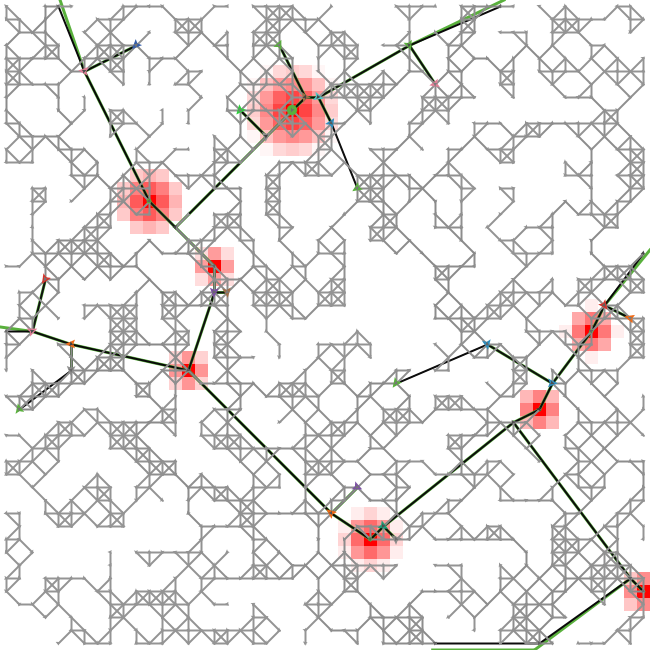
\includegraphics[width=0.48\linewidth]{Figures/NetworkGrowth/example-bio-process-1}}\hspace{0.2cm}
%\frame{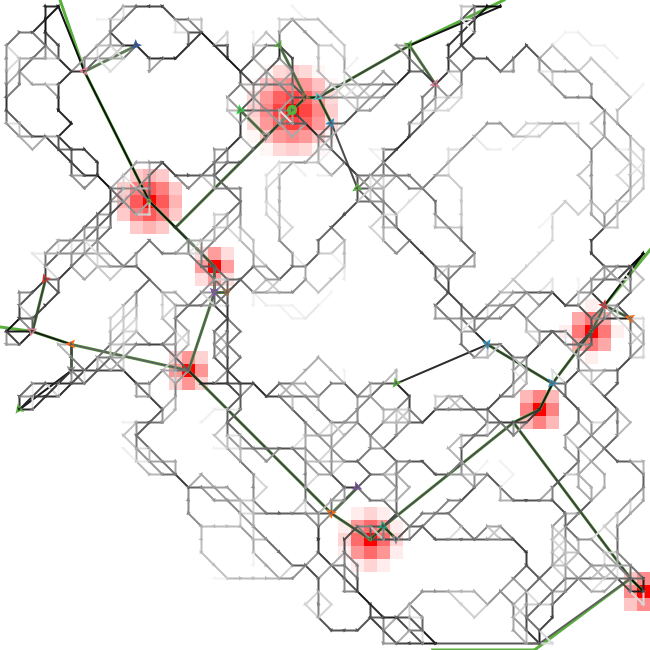
\includegraphics[width=0.48\linewidth]{Figures/NetworkGrowth/example-bio-process-1-tick80}}
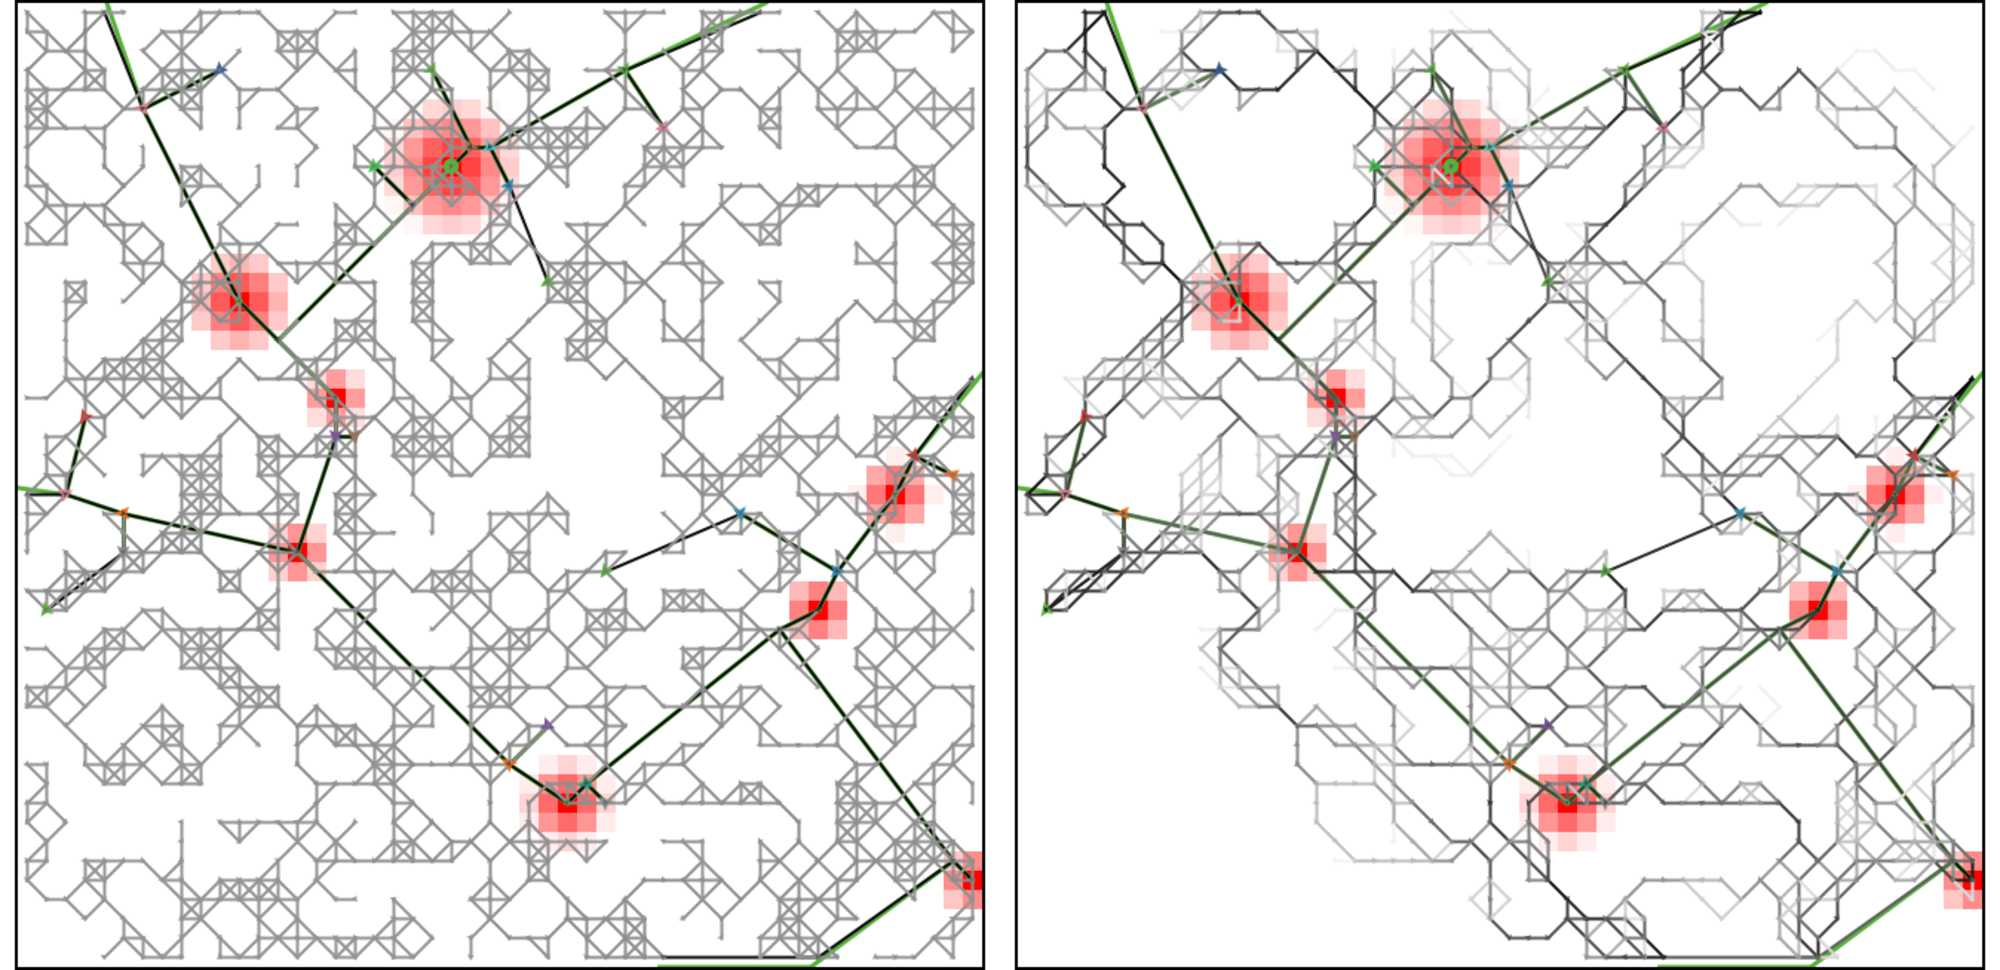
\includegraphics[width=\linewidth]{Figures/Final/7-1-1-fig-networkgrowth-bioexample.jpg}
\caption[Biological Network Example][Exemple de génération de réseau biologique]{\textbf{Biological heuristic for network generation.}\label{fig:networkgrowth:bioexample}}{\textbf{Heuristique biologique pour la generation de réseau.} Cet exemple de visualisation illustre les étapes intermédiaires pour l'ajout de lien. \textit{(Gauche)} le réseau semi-aléatoire initial dans lequel le slime mould est lancé ; \textit{(Droite)} Même réseau après 80 itérations du slime mould, l'épaisseur des liens donnant la capacité.\label{fig:networkgrowth:bioexample}}
\end{figure}
%%%%%%%%%%%%%%%%%


%%%%%%%%%%%%%%%%%%%%%%%
\subsubsection{Cost-benefits heuristic}{Evaluation coûts-bénéfices}

La notion de cout n'est pas présente de manière explicite dans l'ensemble des heuristiques de croissance presentees jusqu'ici - elle l'est de manière implicite dans les potentiels de gravité par le paramètre d'attenuation de la distance, ainsi que dans le slime-mould puisque celui-ci génère des réseau compromis entre robustesse et cout. Nous ajoutons donc une heuristique simple qui est centrée sur le cout des tronçons de réseau lors de leur extension. Il s'agit de celle étudiée par~\cite{louf2013emergence}, qui se base sur des arguments d'économie des transports. Suivant une logique d'analyse coûts-bénéfices par les acteurs du développement du réseau, les liens sont réalisés séquentiellement pour les couples de villes non-connectées ayant un coût minimal, avec un coût de la forme $d_{ij} - \lambda / V_{ij}$, où le paramètre $\lambda$ est le compromis entre coût de construction et gain de potentiel connecté.


% Bien que les problèmes d'évaluation des infrastructures de transport ne puissent se ramener à une simple équation économique unidimensionnelle, des pratiques d'agrégation linéaire coûts-bénéfices, typiques des méthodes de coûts généralisés dont les ingénieurs en transport sont friands, ont été pratiquées pendant un certain temps et le sont encore aujourd'hui dans certain cas. Cet aspect a été intégré dans un modèle de génération de réseau de manière volontairement naïve par~\cite{louf2013emergence}, qui permet déjà de produire un hiérarchie et une transition de phase dans le réseau de transport. Nous proposons de comparer cette heuristique aux autres afin de voir le rôle du coût qui n'est pas présent explicitement dans celles-ci.



%%%%%%%%%%%%%%%%%%%%%%%
\subsubsection{Parameters}{Paramètres}


Nous résumons les paramètres que nous ferons varier par la suite en Table~\ref{tab:networkgrowth:parameters}. Un ``paramètre'' supplémentaire, ou plutôt un méta-paramètre, est le choix de l'heuristique pour l'ajout des liens.


%%%%%%%%%%%%%%
\begin{table}
\caption[Summary of network growth parameters][Résumé des paramètres de croissance de réseau]{\textbf{Summary of network growth parameters.} with their default values.\label{tab:networkgrowth:parameters}}{\textbf{Résumé des paramètres de croissance de réseau pour l'ensemble des heuristiques.} Nous donnons également les processus correspondant, les bornes typiques de variation et leur valeur par défaut.\label{tab:networkgrowth:parameters}}
\begin{tabular}{|c|c|c|c|c|c|}
  \hline
Heuristique & Paramètre & Nom & Processus & Domaine & Défaut\\
  \hline
\multirow{5}{*}{Base}& $l_m$ & liens ajoutés & croissance & $[0;100]$ & $10$ \\\cline{2-6}
 & $d_G$ & distance gravitaire & potentiel & $]0;5000]$ & $500$ \\\cline{2-6}
 & $d_0$ & forme gravitaire & potentiel & $]0;10]$ & $2$ \\\cline{2-6}
 & $k_h$ & poids gravitaire & potentiel & $[0;1]$ & $0.5$ \\\cline{2-6}
 & $\gamma_G$ & hiérarchie gravitaire & potentiel & $[0.1;4]$ & $1.5$ \\\hline
\multirow{2}{*}{Rupture aléatoire}& $\gamma_R$ & hiérarchie aléatoire & hiérarchie & $[0.1;4]$ & $1.5$ \\\cline{2-6}
& $\theta_R$ & seuil aléatoire & rupture & $[1;5]$ & $2$ \\\hline
Coût-Bénéfices& $\lambda$ & seuil aléatoire & compromis & $[0;0.1]$ & $0.05$ \\\hline
\multirow{2}{*}{Biologique}& $n_b$ & itérations & convergence & $[40;100]$ & $50$ \\\cline{2-6}
& $\theta_b$ & seuil biologique & seuil & $[0.1;1.0]$ & $0.5$ \\\hline
\end{tabular}
\end{table}
%%%%%%%%%%%%%%






%%%%%%%%%%%%%%%%%%%%%%%
\subsection{Results}{Résultats}


\subsubsection{Model setup}{Initialisation du modèle}

Le modèle est initialisé sur configuration synthétiques ou semi-synthétiques :
\begin{enumerate}
	\item La densité de population est initialisée soit par mélange d'exponentielles, dont les centres (noeuds du réseau) suivent la configuration d'un système de ville synthétique comme fait en~\ref{sec:macrocoevolexplo} (ici paramètres par défaut $\alpha_S = 0.8$) ; soit à partir d'une configuration réelle extraite du raster de densité pour la France. 
	\item Dans le second cas, un nombre fixe de noeud du réseau sont générés et localisés de manière préférentielle selon la densité (voir~\ref{sec:correlatedsyntheticdata})\footnote{Pour éviter les effets de bord d'un réseau n'ayant aucune connexion avec l'extérieur, nous ajoutons un nombre fixe $n_e$ de noeuds (que nous prenons $n_e = 6$) à des points aléatoires sur le bord du monde.}. Nous n'initialisons pas sur réseau réel puisqu'il s'agira de la cible de calibration, mais imposons un squelette initial synthétique pouvant être interprété comme un réseau archaïque.
	\item Un réseau initial est créé par connection des noeuds comme détaillé en~\ref{sec:correlatedsyntheticdata}.
\end{enumerate}


\subsubsection{Generated networks}{Réseaux générés}

Une illustration visuelle des différentes topologies générées est donnée en Fig~\ref{fig:networkgrowth:examples}. Cela permet de comparer les particularité de chacune des heuristiques. Par exemple, les liens formés par la rupture aléatoire en comparaison à la rupture déterministe témoignent de la dépendance au chemin et produisent un réseau moins redondant, tandis que la rupture déterministe renforce le lien le plus fort entre les deux grandes villes proches. L'heuristique basée sur le coût donne des réseaux denses de manière très localisées, mais évite les liens trop longs. Enfin, l'heuristique biologique produit un maillage dense dans la sous-région où les interactions sont les plus fortes.



%%%%%%%%%%%%%%%%%
\begin{figure}
	% example_comp_nwSize200_setup.png
	%\frame{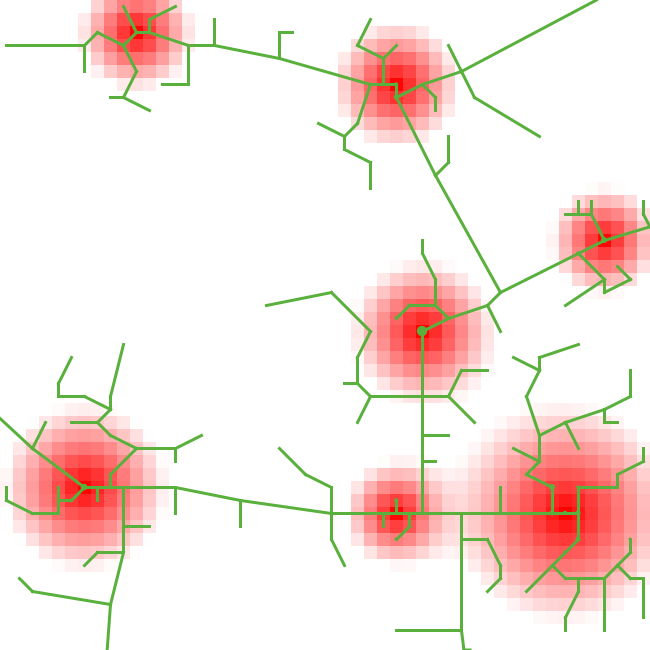
\includegraphics[width=0.32\linewidth]{Figures/NetworkGrowth/example_comp_nwSize200_connex.png}}
	%\frame{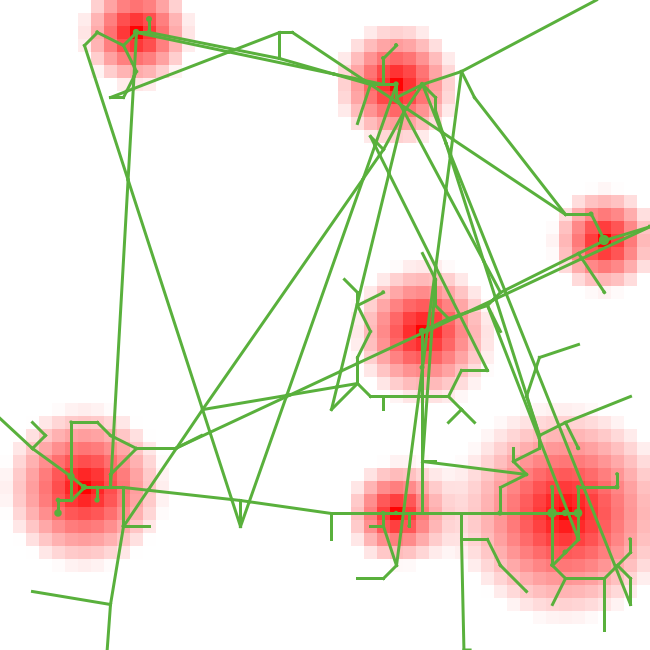
\includegraphics[width=0.32\linewidth]{Figures/NetworkGrowth/example_comp_nwSize200_random.png}}
	%\frame{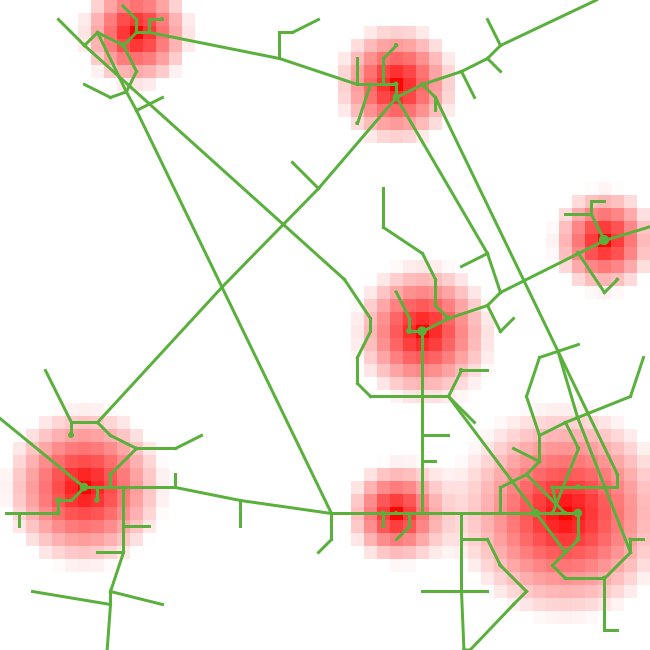
\includegraphics[width=0.32\linewidth]{Figures/NetworkGrowth/example_comp_nwSize200_rndbrkdwn.png}}\\
	%\frame{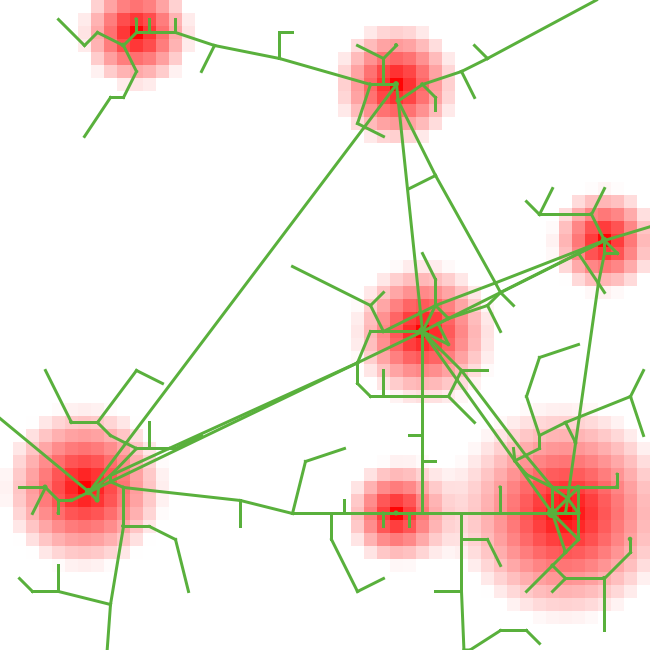
\includegraphics[width=0.32\linewidth]{Figures/NetworkGrowth/example_comp_nwSize200_detbrkdwn.png}}
	%\frame{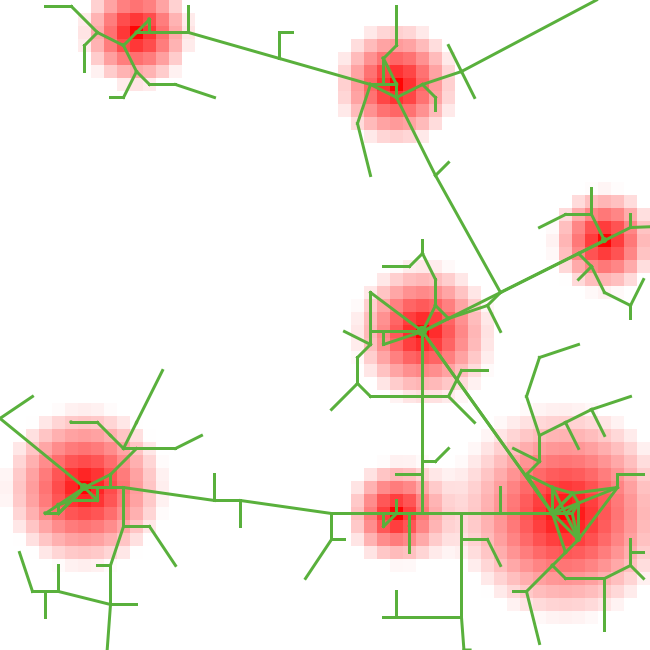
\includegraphics[width=0.32\linewidth]{Figures/NetworkGrowth/example_comp_nwSize200_cost.png}}
	%\frame{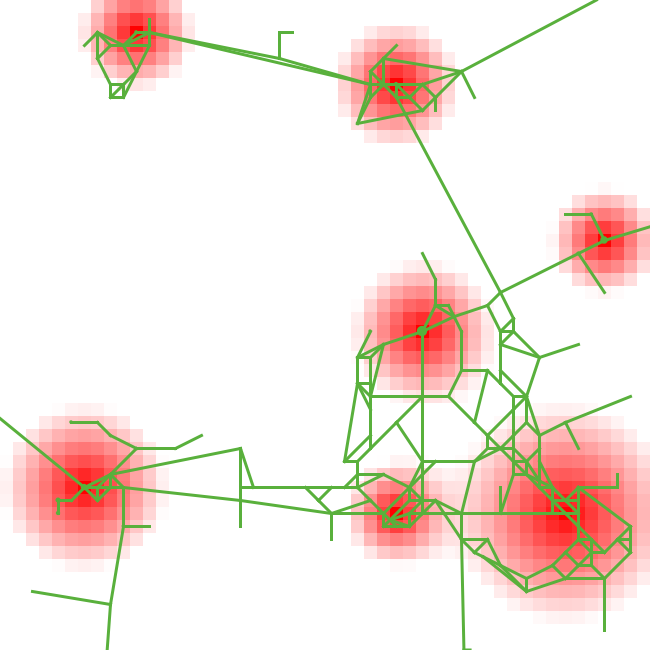
\includegraphics[width=0.32\linewidth]{Figures/NetworkGrowth/example_comp_nwSize200_bio.png}}
	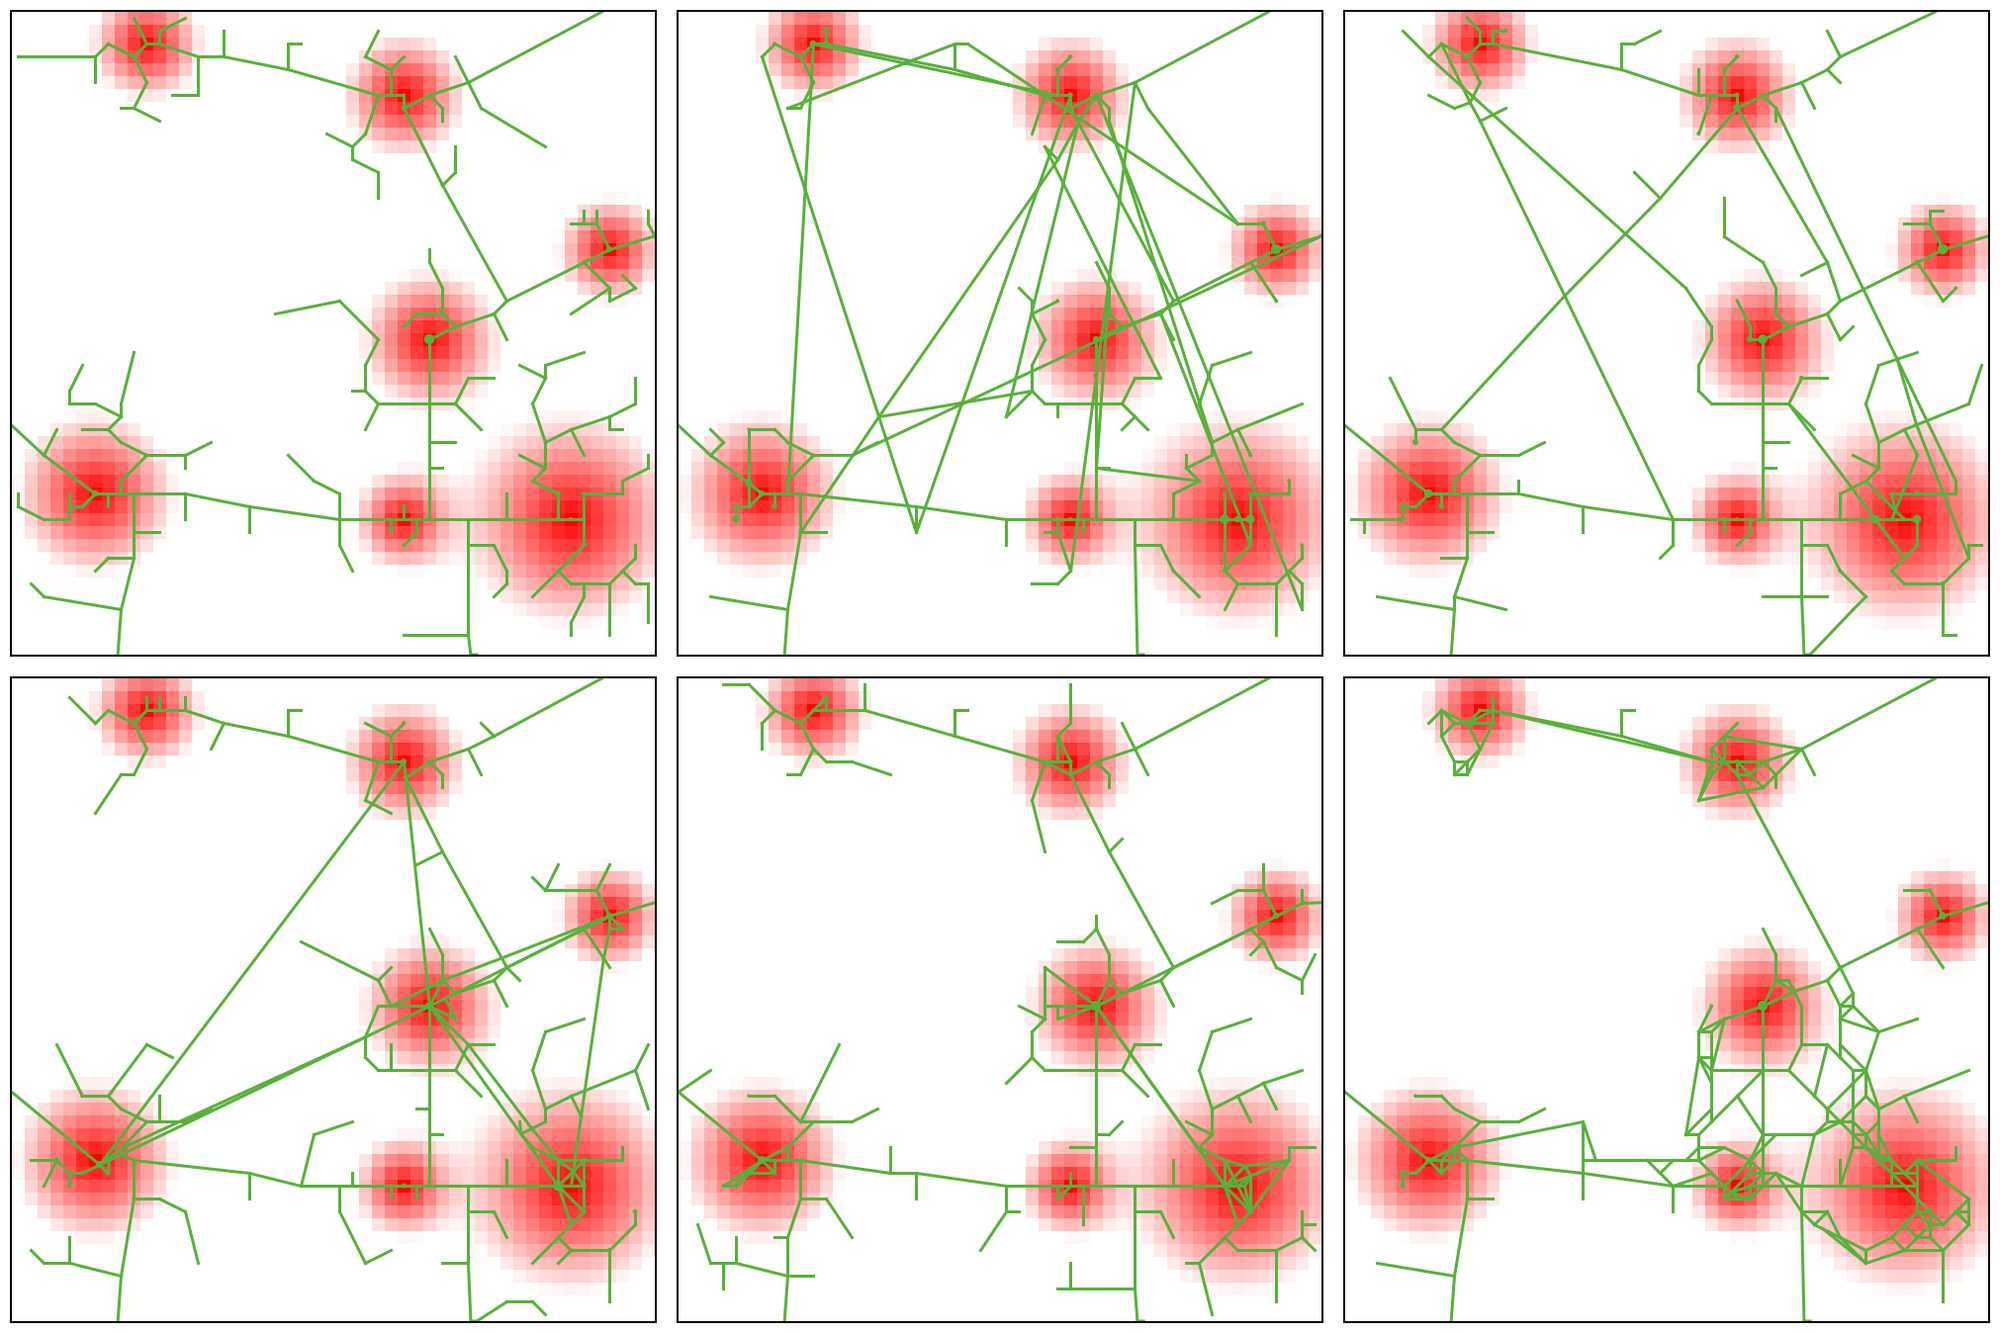
\includegraphics[width=\linewidth]{Figures/Final/7-1-2-fig-networkgrowth-examples.jpg}
\caption[Network examples][Exemples de réseaux]{\textbf{Examples of networks obtained with the different heuristics.}\label{fig:networkgrowth:examples}}{\textbf{Exemples de réseaux obtenus par les différentes heuristiques.} Les réseaux sont obtenus pour une même configuration de densité composée de 7 centres, et du même réseau initial les reliant. Nous prenons $l_m = 10$ et fixons la taille finale à 200 noeuds. Les paramètres gravitaires sont $d_G = 2000$, $d_0 = 3$, $\gamma_G = 0.3$, $k_h = 0.6$. Dans l'ordre de gauche à droite et de haut en bas : réseau par connexion seule ; réseau aléatoire ; rupture de potentiel aléatoire avec $\gamma_R = 2$ et $\theta_R = 1.6$ ; rupture de potentiel déterministe ; coût bénéfice avec $\lambda = 0.009$ ; biologique avec $n_b = 50$ et $\theta_b = 0.6$.\label{fig:networkgrowth:examples}}
\end{figure}
%%%%%%%%%%%%%%%%%

% Nous fixons ici $n_N = 100$.



\subsubsection{Experience plan}{Plan d'expérience}


Détaillons un plan d'expérience pour explorer l'espace des réseaux générés par les différentes heuristiques. La génération de réseau est faite à densité de population constante, sur configurations réelles classifiées morphologiquement en~\ref{sec:staticcorrelations}. Nous considérons 50 grilles réelles de densité, correspondant à des zones en France, classées dans 5 classes morphologiques. La description de celles-ci est donnée en Annexe~\ref{app:sec:networkgrowth}, et montre qu'elle couvrent un ensemble de morphologies allant d'établissements très localisés et dispersés à des structures polycentriques, et des configurations intermédiaires.

%       moran  distance   entropy     slope rsquaredslope
%1 0.2324194 0.6580061 0.7590965 0.6202700     0.8673209
%2 0.4748752 0.5024231 0.7516852 0.5305178     0.8307633
%3 0.2133188 0.4208907 0.5745856 0.6520814     0.8107935
%4 0.2354844 0.7482191 0.8994017 0.8677689     0.7508533
%5 0.1505684 0.7604514 0.8418746 0.7168180     0.8796809

Etant donné les plages de paramètres données précédemment pour chacune des heuristiques, nous comparons l'espace faisable pour une exploration basique en criblage LHS de l'espace des paramètres, pour l'ensemble des grilles de densité, avec 5 répétitions par point de paramètre\footnote{Correspondant à environ 240,000 répétitions du modèle. Le jeu de données issu des simulation est disponible à \url{http://dx.doi.org/10.7910/DVN/OBQ4CS}.}.

\subsubsection{Feasible space}{Topologies obtenues}

Les réseaux sont caractérisés ici par les indicateurs suivants : centralité de chemin moyenne $\bar{bw}$ et centralité de proximité moyenne $\bar{cl}$, diamètre $r$, longueur moyenne de chemin $\bar{l}$, vitesse relative $v_0$. Pour visualiser les espaces faisables et les comparer aux réseaux réels par la suite, nous réduisons l'espace dans un hyperplan principal, à partir des points obtenus dans les simulations. La composition des deux premières composantes est la suivante : $PC1 = - 0.51 \bar{bw} - 0.45 \bar{l} + 0.57 v_0 - 0.43 r + 0.05 \bar{cl}$ et $PC2 = -0.45 \bar{bw} + 0.17 \bar{l} +0.33 v_0 + 0.8 r +0.1 \bar{cl}$. La première va caractériser des réseaux où les chemins sont courts, tandis que la deuxième exprime des réseaux à distance moyenne plus grande, donc plus étalés, mais plus efficients en termes de $v_0$. 

 
Le nuage de points de l'espace topologique faisable, obtenu avec le plan d'expérience décrit ci-dessus, est donné en Fig.~\ref{fig:networkgrowth:feasiblespace}. La couverture est permise par la complémentarité des différents nuages pour chaque heuristique. Par exemple, l'heuristique aléatoire est à l'opposée complète de la référence, en termes de la première composante : le réseau arborescent de référence induit logiquement un plus grand nombre de détours, et donc des chemins plus longs. La rupture aléatoire permet de couvrir une grande plage sur $PC1$ et occupe une place privilégiée pour les faibles valeurs de $PC2$.


%summary(gnres$concentration)
%   Min. 1st Qu.  Median    Mean 3rd Qu.    Max. 
% 0.3288  0.5383  0.7551  0.7405  1.0000  1.0000 
% 0.85^2+0.15^2 = 0.745
% 0.65^2+0.35^2 = 0.545

Pour mieux comprendre la complémentarité des approches, on peut quantifier l'intersection des nuages de points de la Fig.~\ref{fig:networkgrowth:feasiblespace} par une méthode simple : en divisant le plan en une grille (qu'on prend de taille 20x20), les proportions $p_{ij}$ de points de chaque heuristique $j$ pour chaque cellule $i$ peuvent être agrégées en un indexe de concentration $h = \sum_i p_i^2$ dont la distribution décrit les équilibres dans les régions de l'espace. On obtient pour les cellules un premier quartile à $0.54$, une médiane à $0.76$ et un troisième quartile à $1$. Pour comparaison, dans le cas de deux types de points seulement, une répartition 65-35\% donne un indice de $0.55$ et une répartition un indice de $0.75$, ce qui veut dire qu'au moins la moitié des cellules ont plus de trois quarts de points dans une unique catégorie. Cela confirme la conclusion de forte complémentarité des heuristiques.


%%%%%%%%%%%%%%%%%
\begin{figure}
%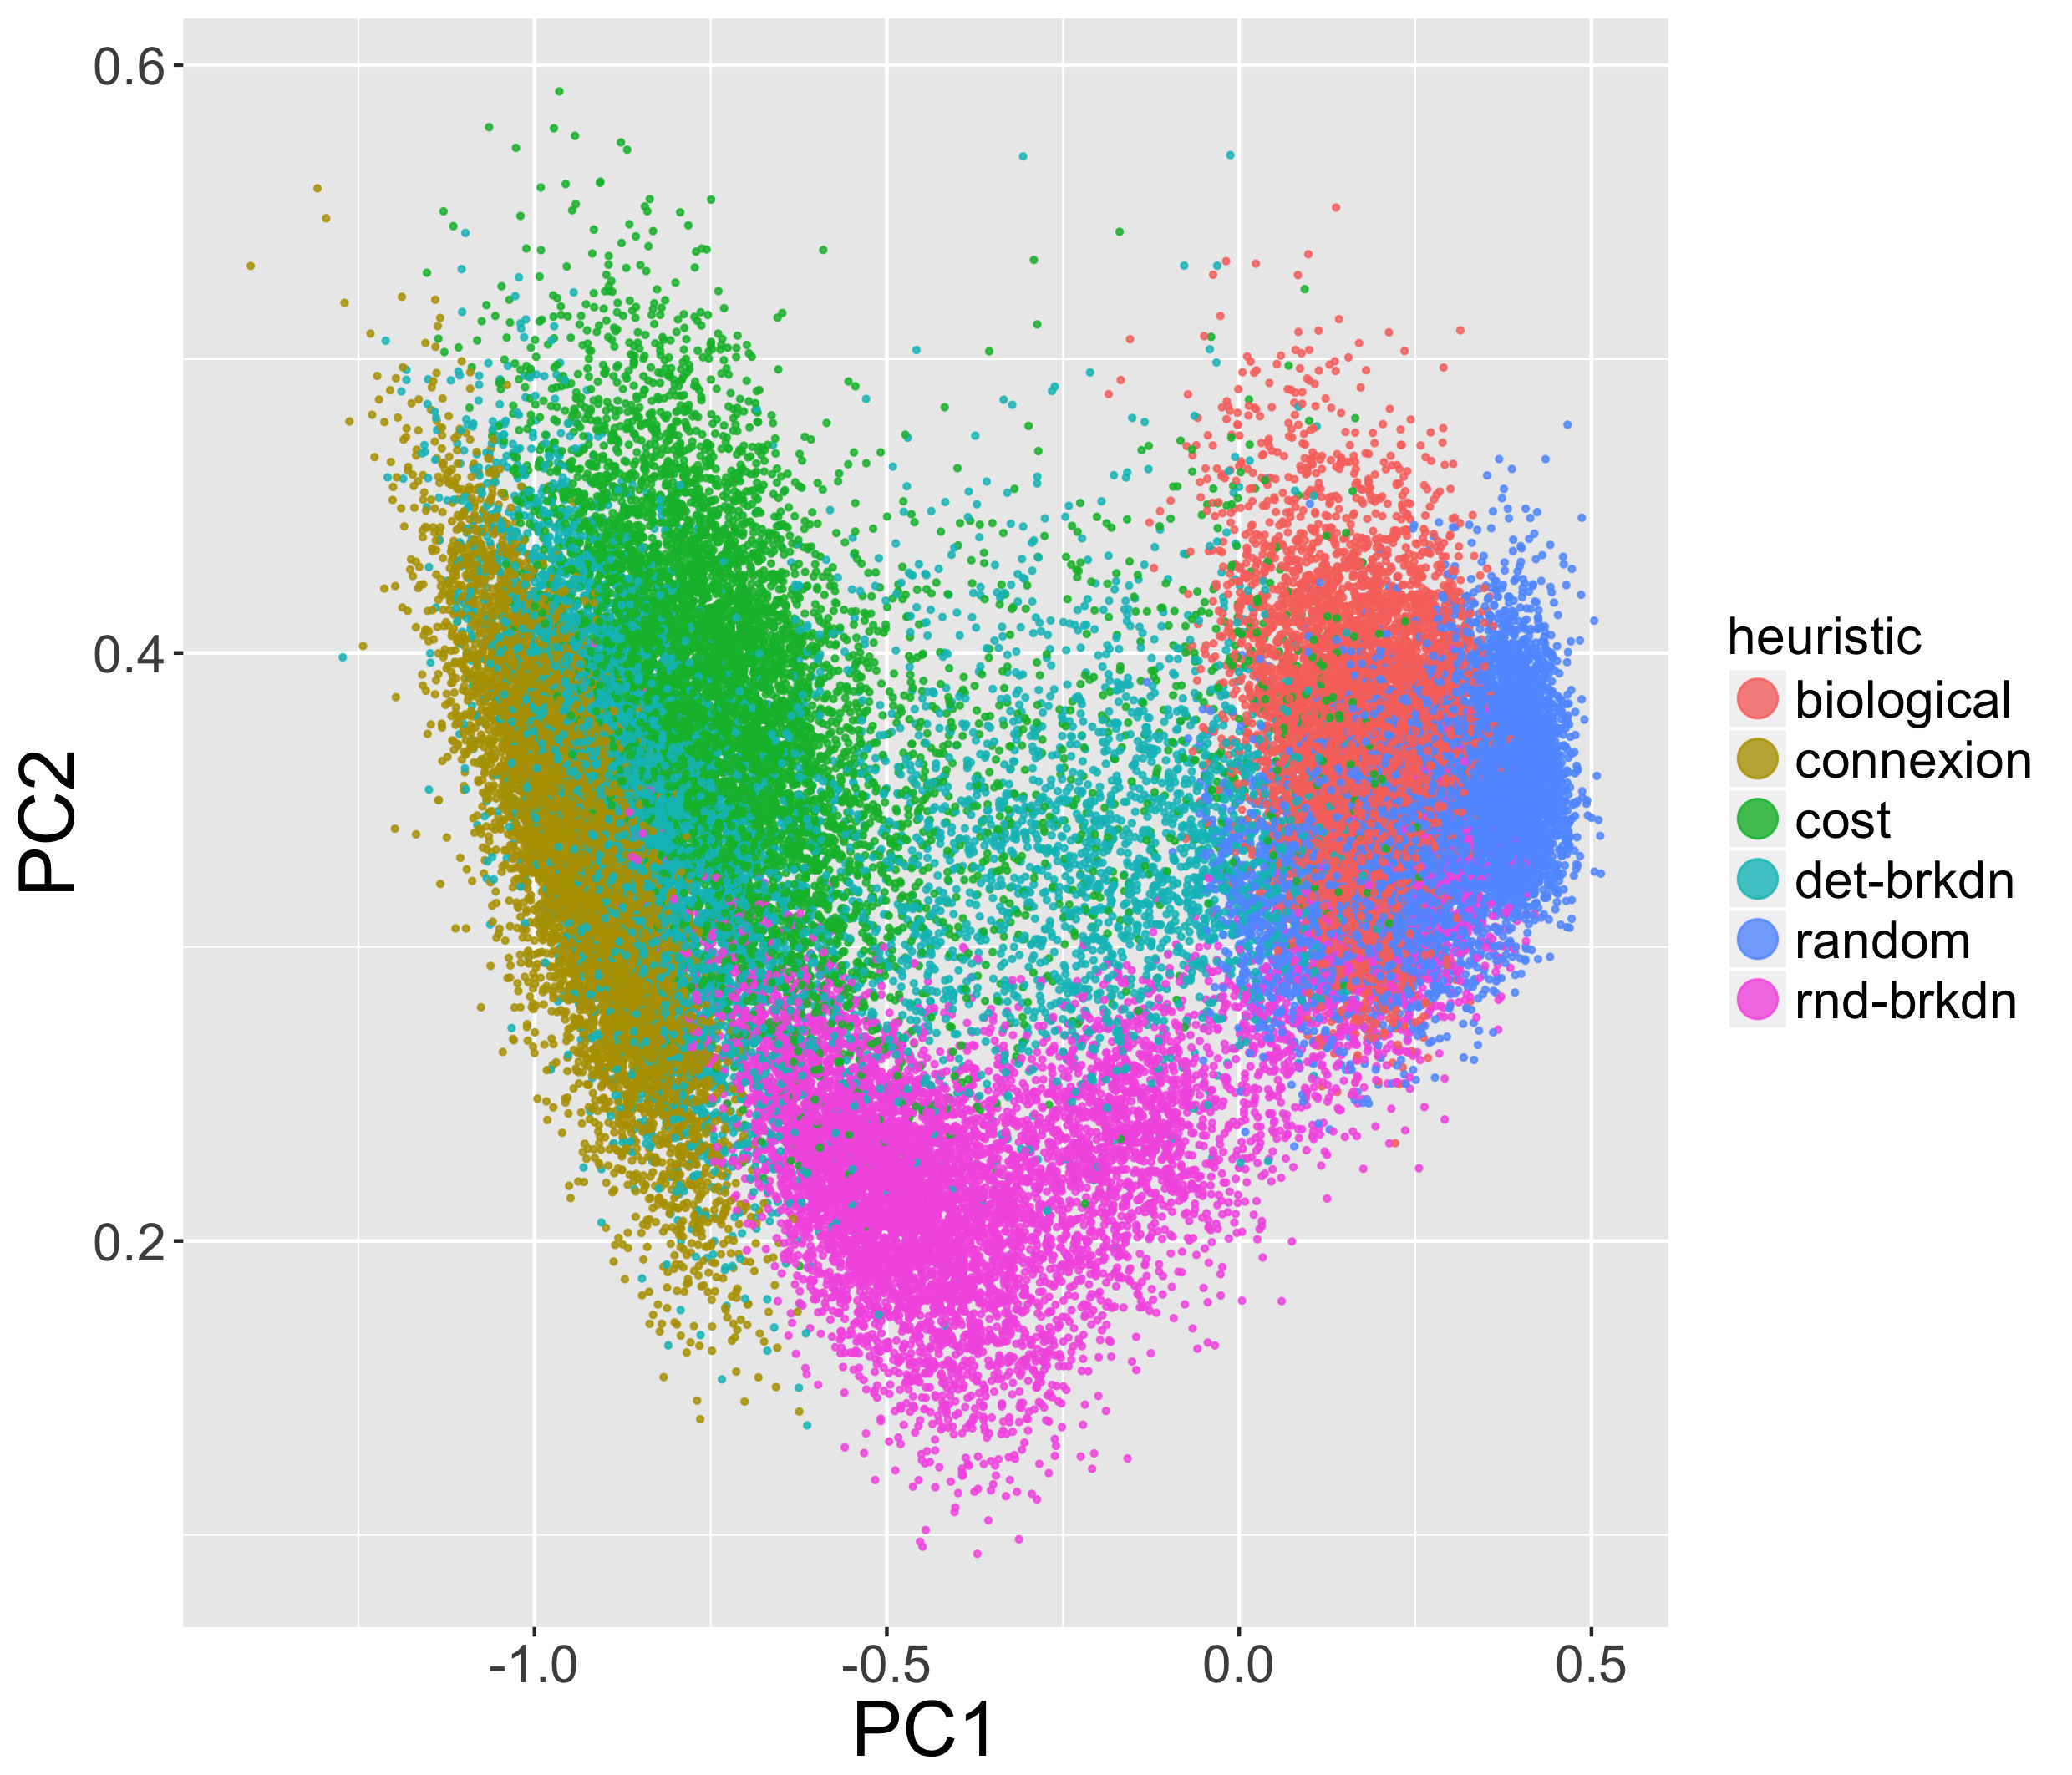
\includegraphics[width=\linewidth]{Figures/NetworkGrowth/feasible_space_pca}
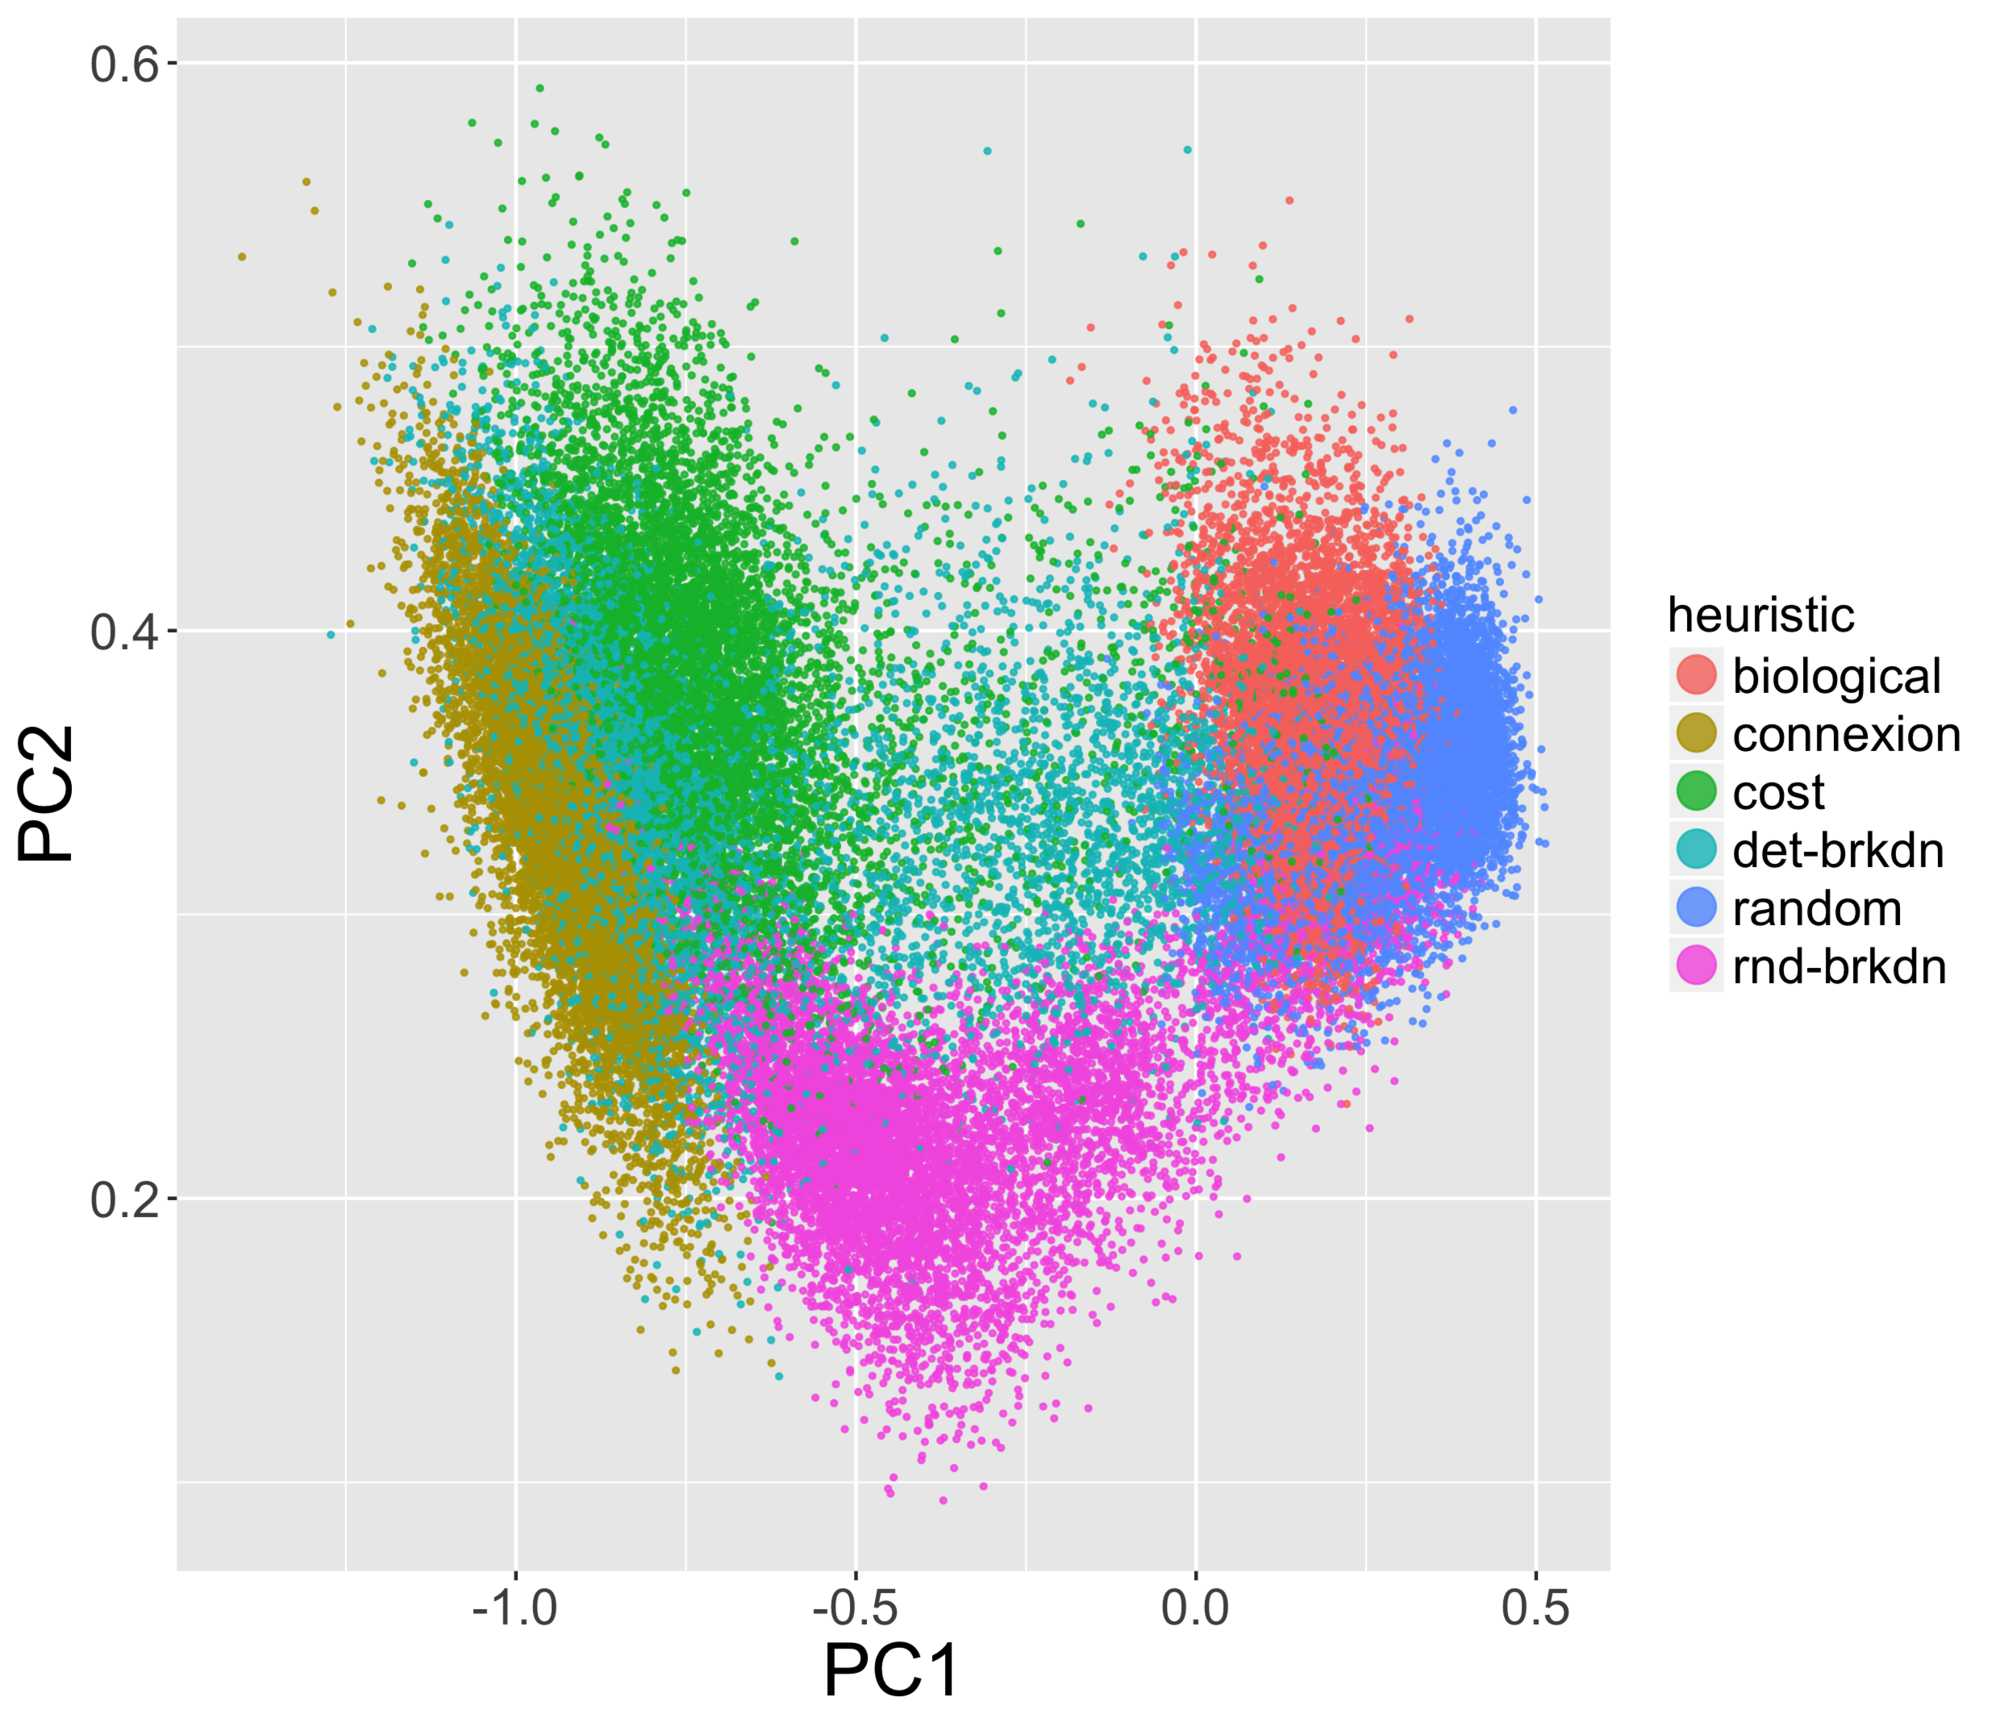
\includegraphics[width=\linewidth]{Figures/Final/7-1-2-fig-networkgrowth-feasiblespace.jpg}
\caption[Feasible topological space][Espace topologique faisable]{\textbf{Feasible topological space.}\label{fig:networkgrowth:feasiblespace}}{\textbf{Espace topologique faisable pour les différentes heuristiques de génération.} Les nuages de points couvrent des régions complémentaires de l'espace topologique. La même figure conditionnée à la classe morphologique de densité est donnée en Appendice~\ref{app:sec:networkgrowth}.\label{fig:networkgrowth:feasiblespace}}
\end{figure}
%%%%%%%%%%%%%%%%%

% PCA synth
%
%                                PC1        PC2        PC3        PC4         PC5
%meanBwCentrality        -0.51420330 -0.4500671  0.5415210 -0.4602950  0.16708710
%meanPathLength          -0.45662839  0.1782617 -0.2556133  0.3151101  0.77141477
%meanRelativeSpeed        0.57854267  0.3344679  0.3147784 -0.4083421  0.53627500
%nwDiameter              -0.43570261  0.8011179  0.1305644 -0.2508956 -0.29728372
%meanClosenessCentrality  0.05036956  0.1095611  0.7247651  0.6776003 -0.03213514
%Importance of components:
%                          PC1     PC2     PC3     PC4     PC5
%Standard deviation     0.4981 0.06762 0.04611 0.03423 0.02982
%Proportion of Variance 0.9659 0.01780 0.00828 0.00456 0.00346
%Cumulative Proportion  0.9659 0.98370 0.99198 0.99654 1.00000



\subsubsection{Real network comparison}{Comparaison aux réseaux réels}

%%%%%%%%%%%%%%%%%
\begin{figure}
%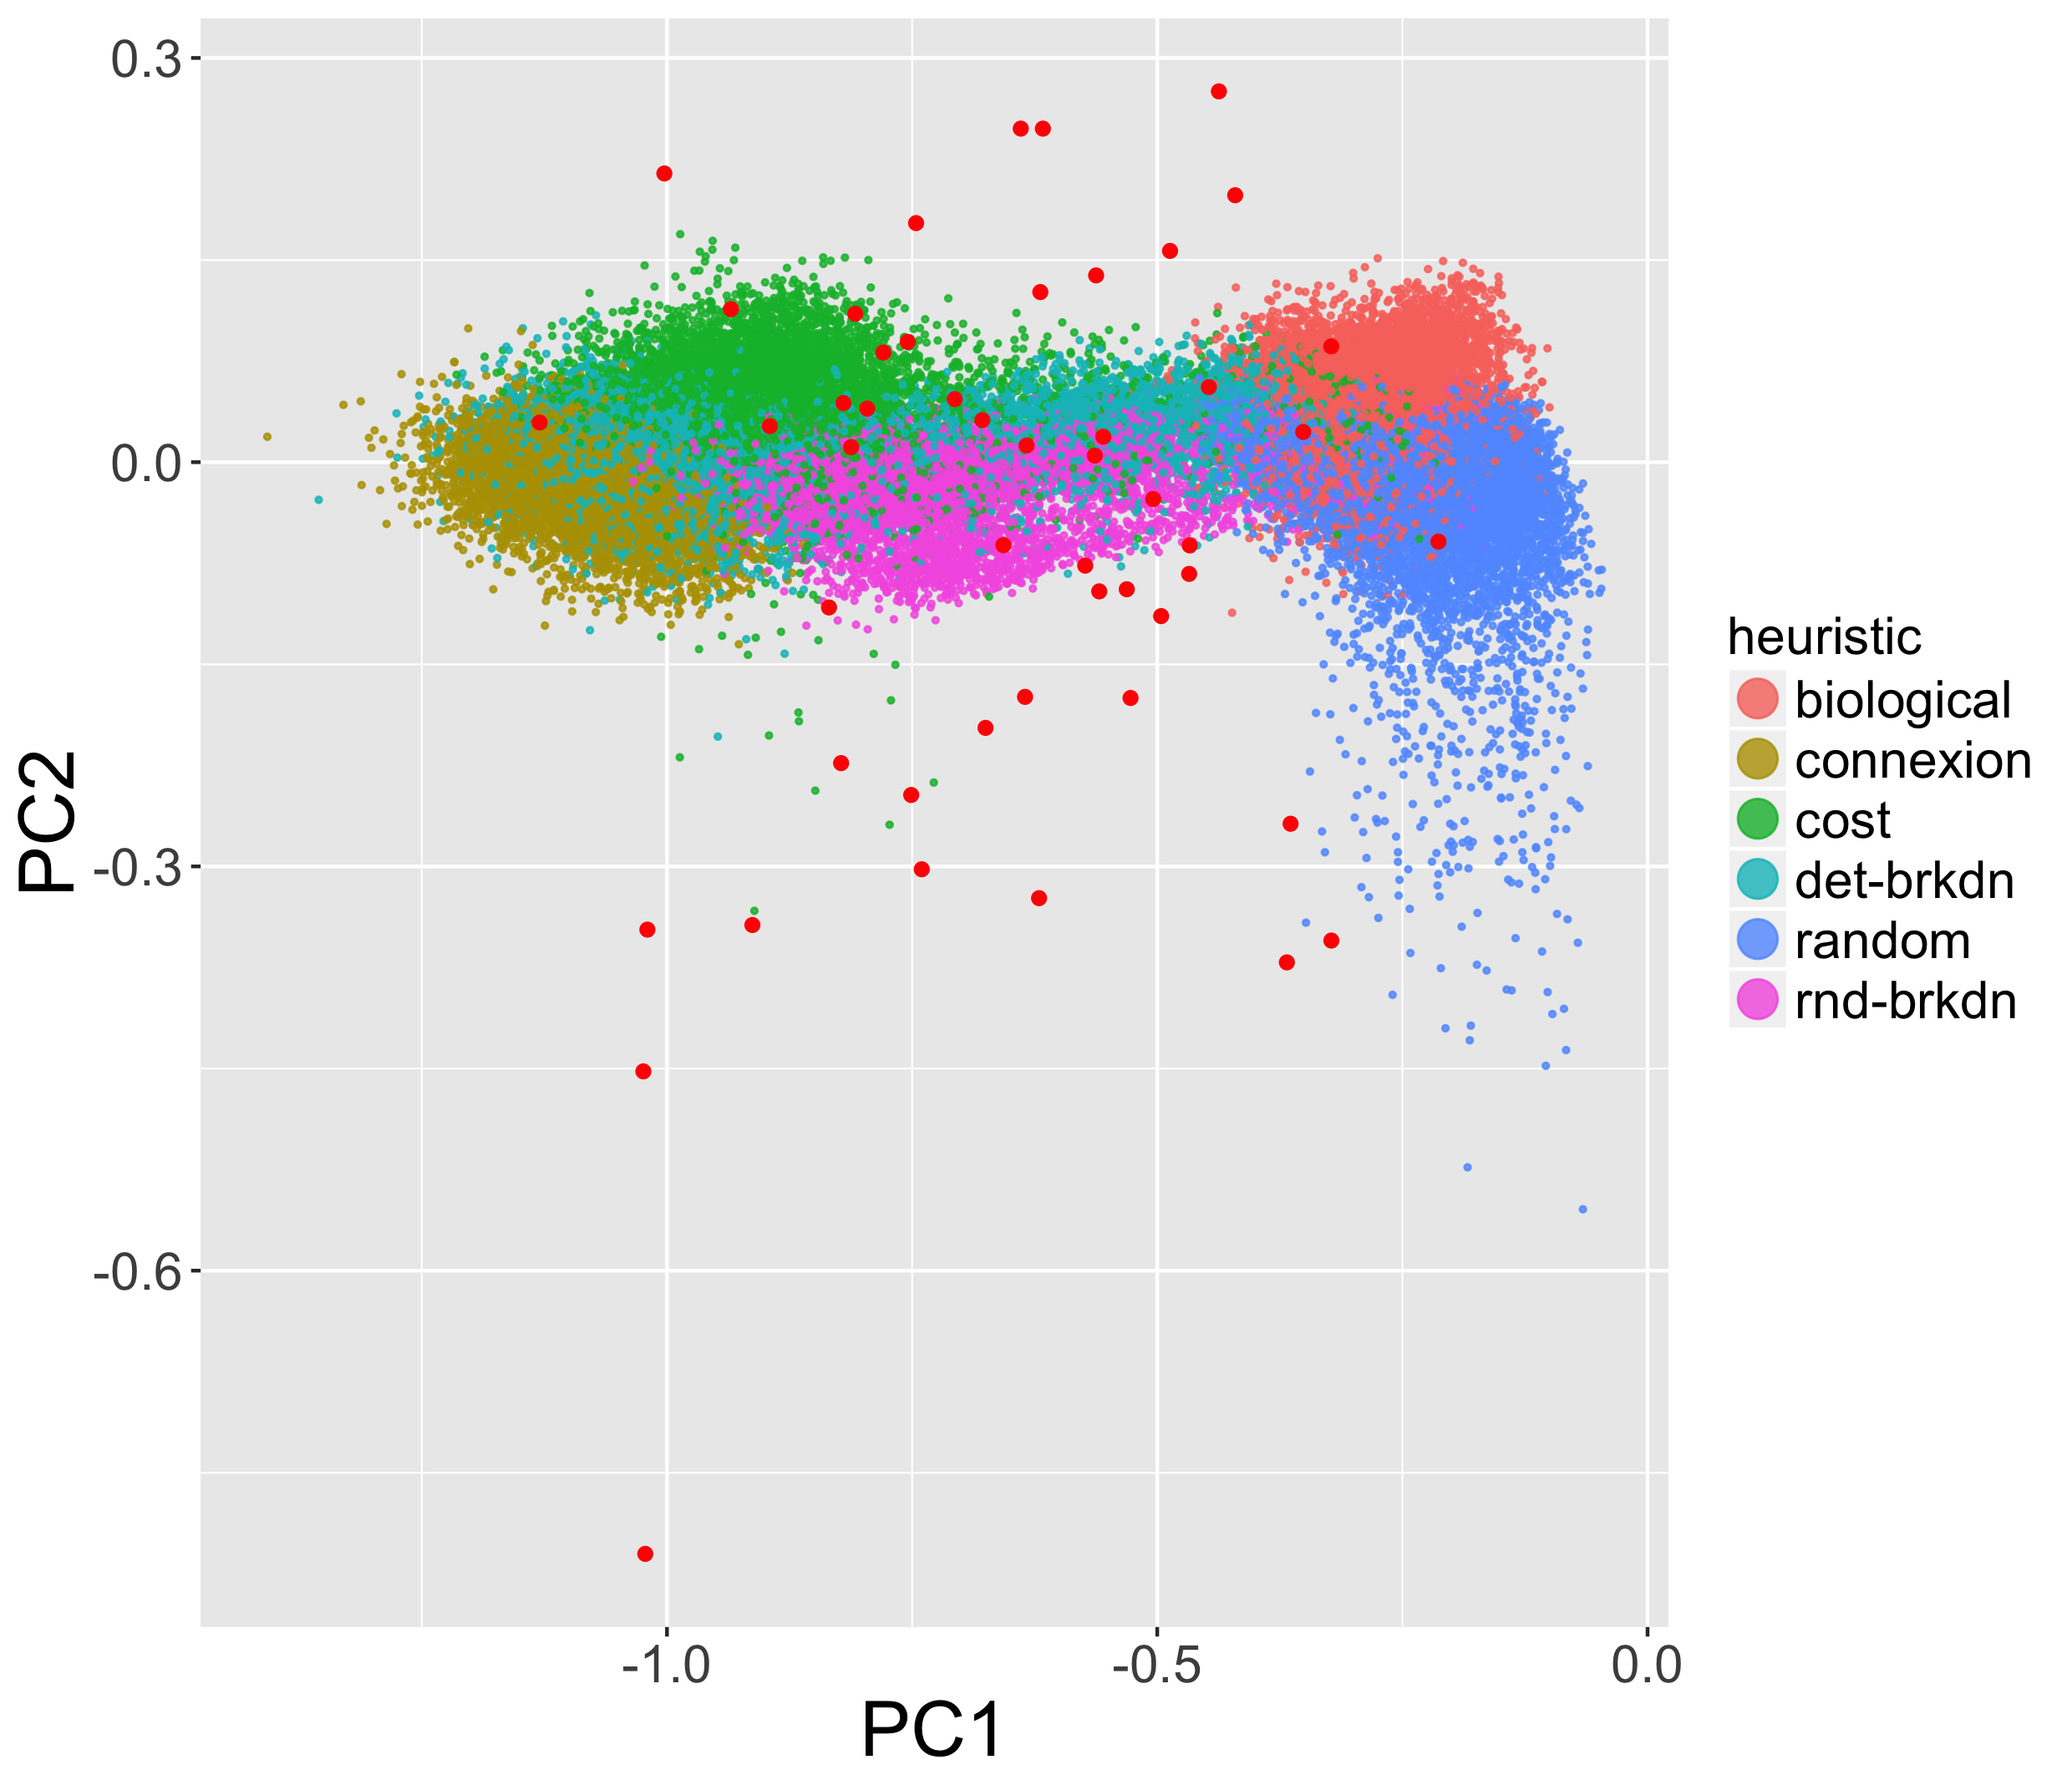
\includegraphics[width=0.45\linewidth]{Figures/NetworkGrowth/feasible_space_withreal_pca}
%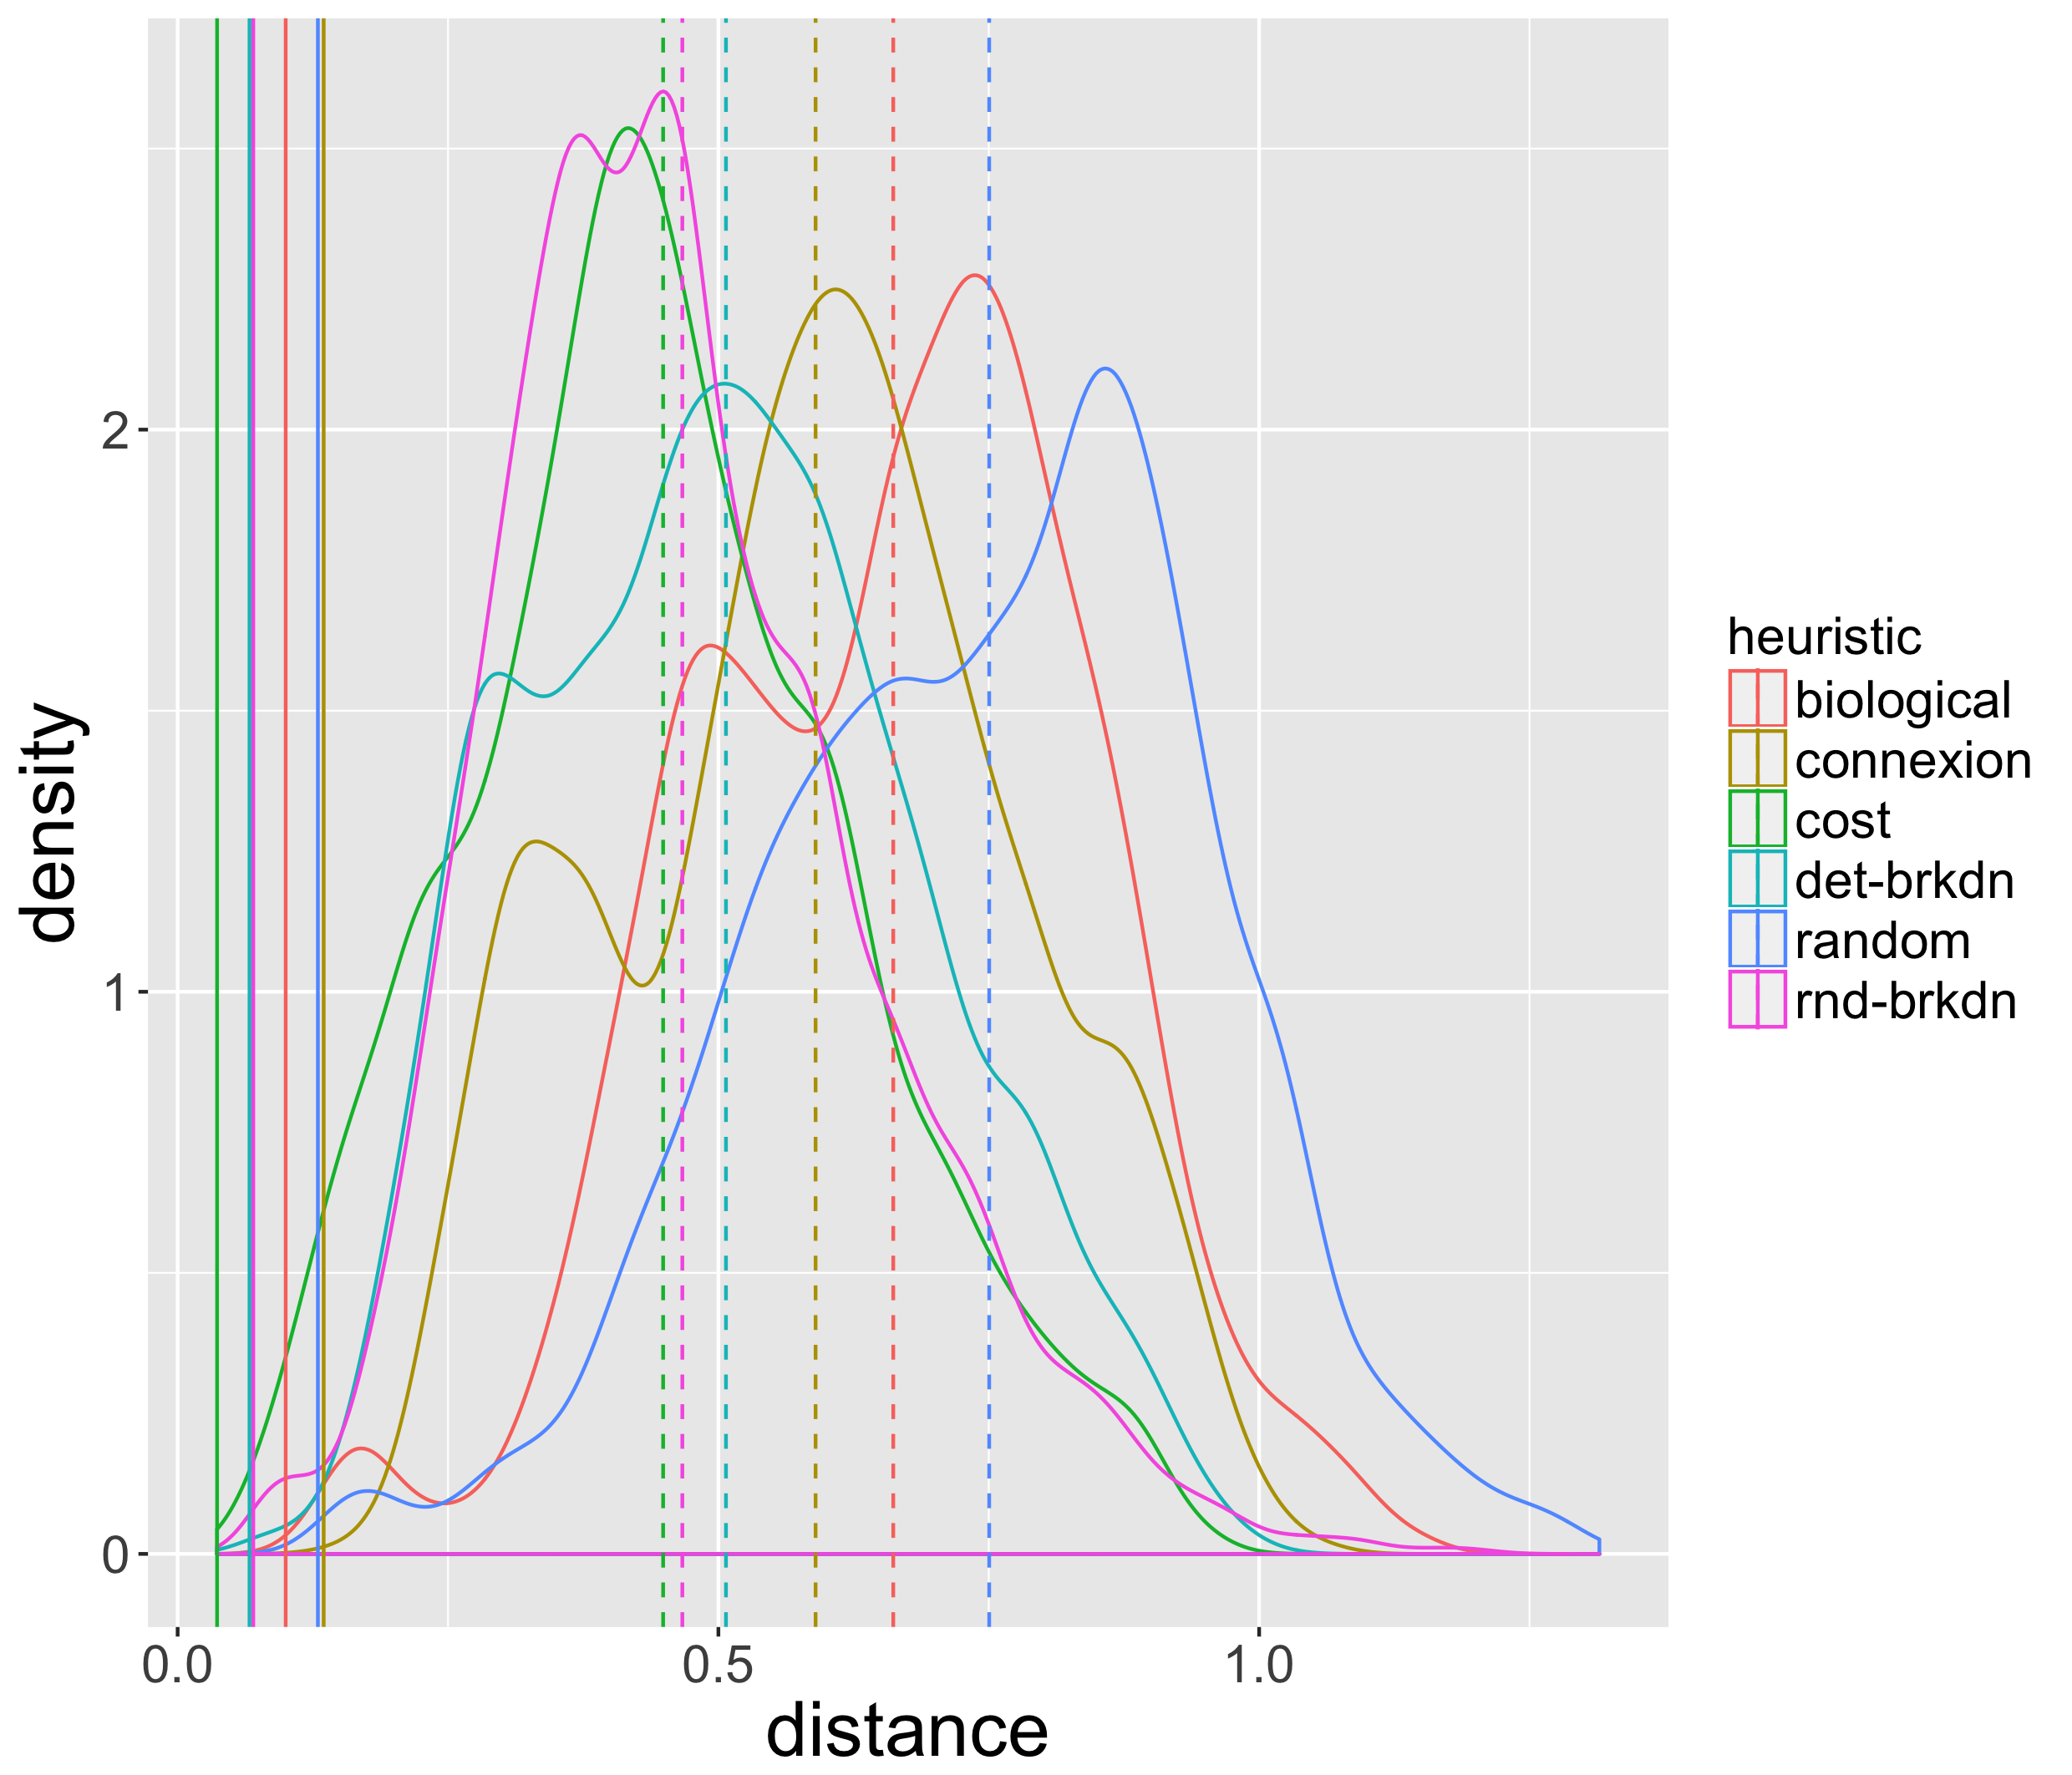
\includegraphics[width=0.45\linewidth]{Figures/NetworkGrowth/distance_real}\\
%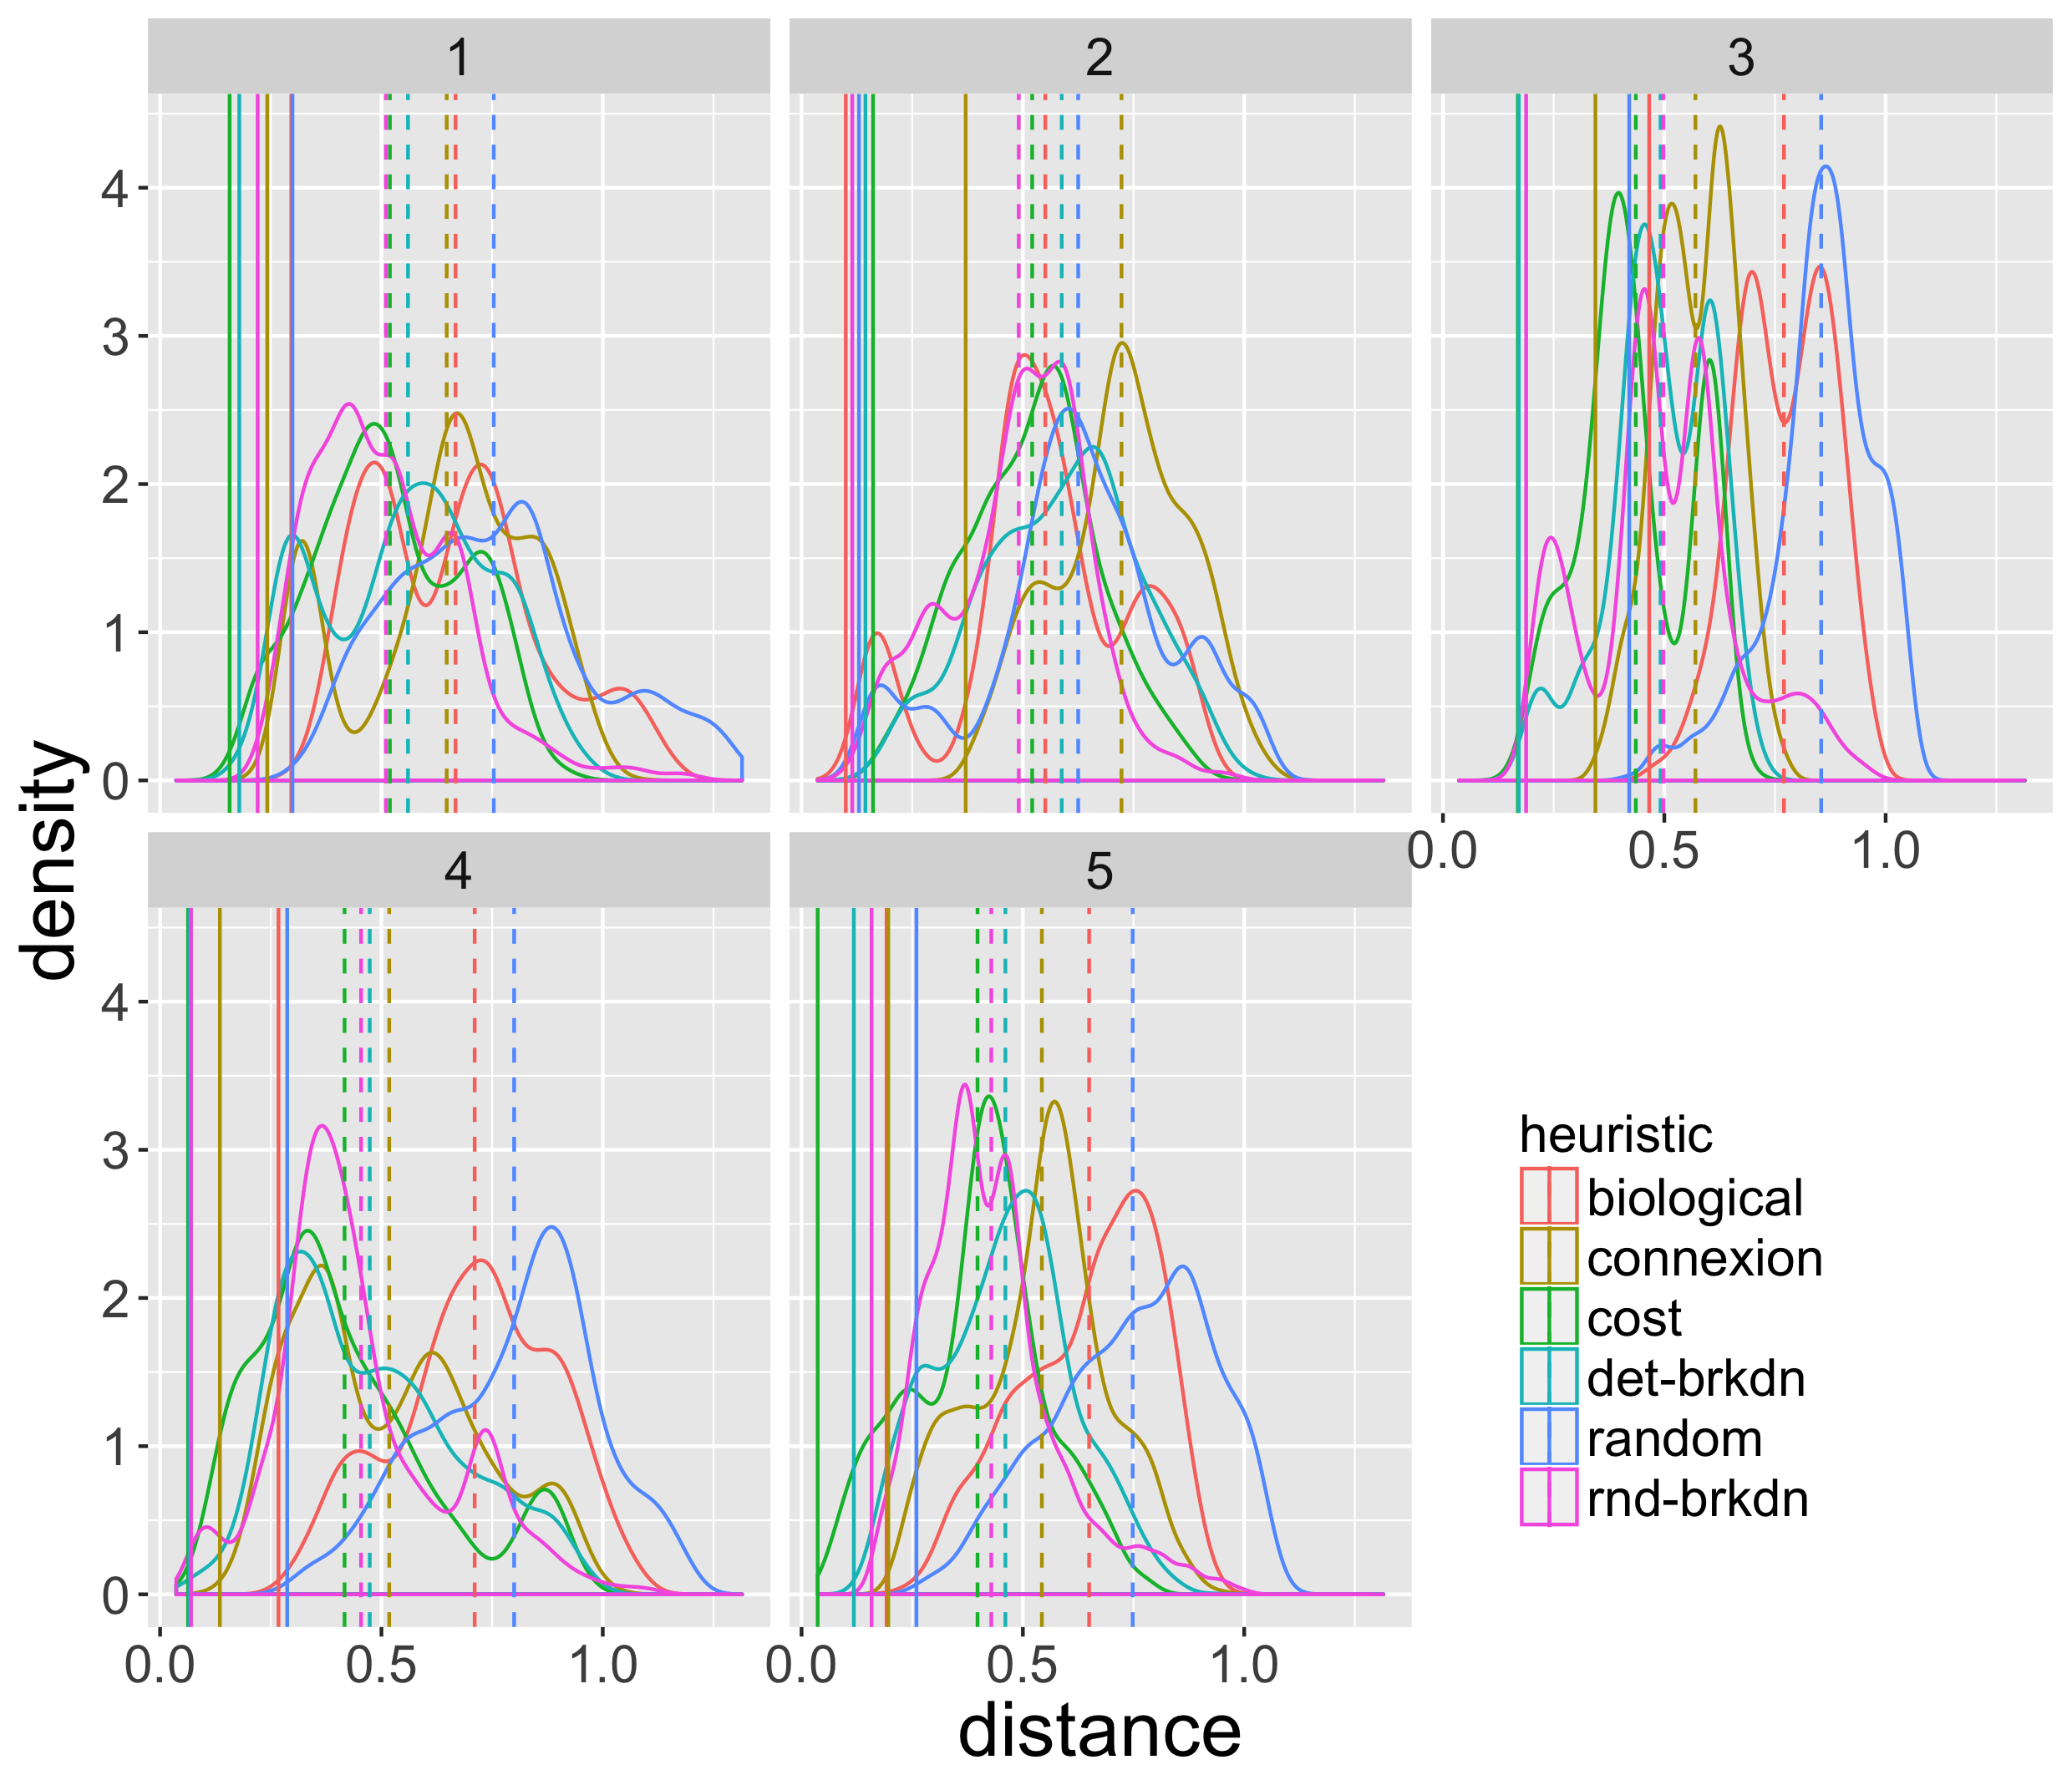
\includegraphics[width=0.8\linewidth]{Figures/NetworkGrowth/distance_real_bymorph}
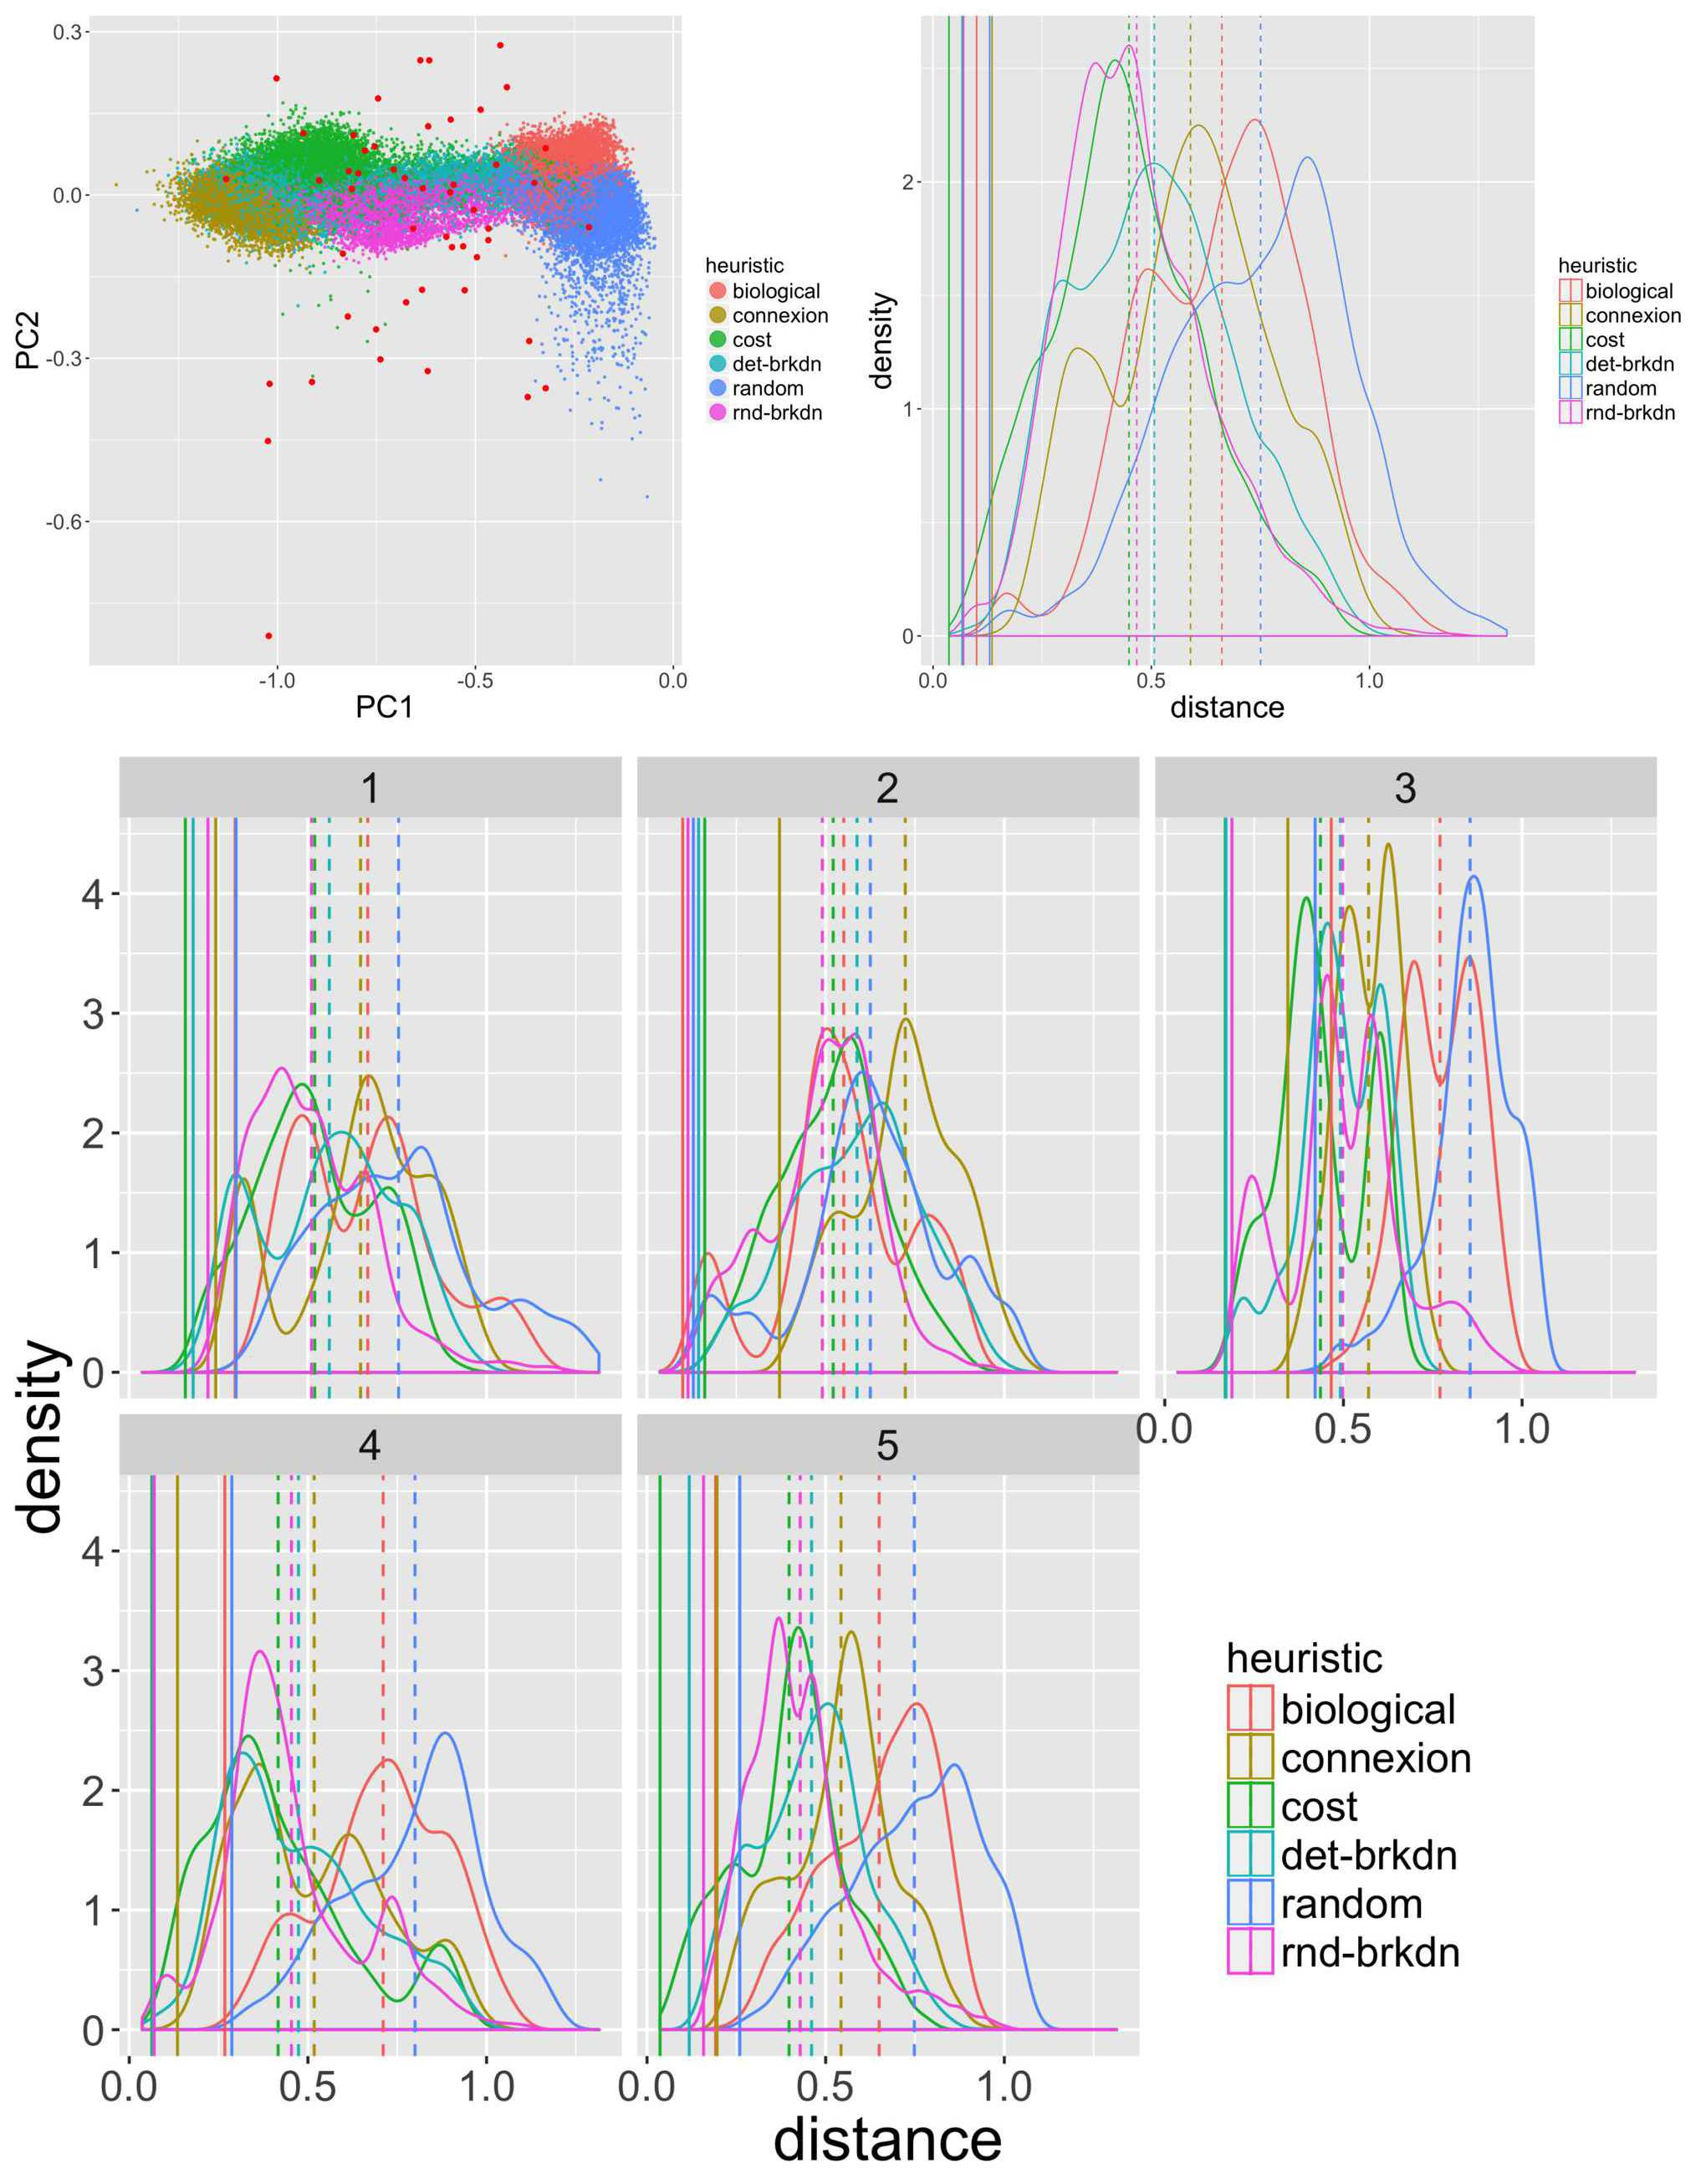
\includegraphics[width=\linewidth,height=0.85\textheight]{Figures/Final/7-1-2-fig-networkgrowth-realdistance}
\caption[Comparison to real networks][Comparaison aux réseaux réels]{\textbf{Comparison to real networks.}\label{fig:networkgrowth:realdistance}}{\textbf{Comparaison aux réseaux réels.} (\textit{Haut Gauche}) Nuage de point des configurations simulées (couleur en légende) et des configurations réelles (en rouge), dans un plan principal tel que $PC1 = 0.12 \bar{bw} - 0.09 \bar{cl} + 0.98 \bar{l}$ et $PC2 = -0.20 \bar{bw} - 0.97 \bar{cl} - 0.06 \bar{l}$. (\textit{Haut Droite}) Distribution des distances $d_{min}$ pour l'ensemble des points simulés, par heuristique (couleur). Les lignes verticales pointillées donnent la moyenne et les lignes solides le minimum pour chaque distribution. (\textit{Bas}) Mêmes histogrammes, conditionnés par classe morphologique pour la distribution de densité.\label{fig:networkgrowth:realdistance}}
\end{figure}
%%%%%%%%%%%%%%%%%


Nous utilisons les mesures sur réseaux routiers réels calculées en~\ref{sec:staticcorrelations} pour calculer une distance des configurations générées aux configurations observées, en considérant les réseaux réels correspondant aux configurations de densité utilisées pour l'initialisation. Nous prenons pour un point de paramètre le minimum de distance euclidienne sur les vecteurs d'indicateurs pour l'ensemble des points réels\footnote{C'est à dire si $d(1,2) = \sqrt{(\bar{bw}_1 - \bar{bw}_2)^2 + (\bar{cl}_1 - \bar{cl}_2)^2 + (\bar{l}_1 - \bar{l}_2)^2}$, on considère $d_{min} = \min_j d(S,R_j)$ si $S$ est le point simulé et $R_j$ l'ensemble des points réels. Nous conservons ici uniquement les indicateurs $\bar{bw}$, $\bar{cl}$ et $\bar{l}$, pour des raisons de normalisation.}. Cette comparaison est possible car les indicateurs sont normalisés.


Les résultats de comparaisons aux points réels sont donnés en Fig.~\ref{fig:networkgrowth:realdistance}. Nous donnons une représentation en nuage de points et les histogrammes de distribution des distances, sur l'ensemble des grilles et par classe morphologique. On constate qu'une dizaine de configurations réelles (1/5ème) se retrouvent à grande distance du nuage de points simulés, mais que les autres tombent à distance faible ou à l'intérieur du nuage de point. Encore une fois, les différentes heuristiques sont complémentaires pour approcher un plus grand nombre de points. Concernant les distances, l'aléatoire est le plus mauvais en termes de mode et de moyenne, suivi par le biologique, la référence (connection), la rupture déterministe puis la rupture aléatoire et le coût qui sont à peut près équivalentes. Chacune réalisent des distances minimales très faibles.


En conditionnant par les classes morphologiques, nous voyons que les classes 3, 4 et 5 donnent le plus de difficultés à l'ensemble des heuristiques en termes de minimum - hors il s'agit des configurations avec établissements très localisés ou population diffuse (voir~\ref{app:sec:networkgrowth}) : il est donc plus facile de reproduire les configurations réelles de réseau dans le cas de structures polycentriques. Dans tous les cas, l'heuristique biologique est peu performante, mais il n'est pas directement possible de savoir si cela est du à sa sous-exploration et aux paramètres fixés ou à sa dynamique intrinsèque.






% PCA full
%Rotation:
%                               PC1         PC2        PC3
%meanBwCentrality         0.1232342 -0.20841025 -0.9702466
%meanPathLength           0.9881203 -0.06469639  0.1394013
%meanClosenessCentrality -0.0918241 -0.97589935  0.1979616
%Importance of components:
%                          PC1     PC2     PC3
%Standard deviation     0.1676 0.02884 0.01203
%Proportion of Variance 0.9664 0.02860 0.00498
%Cumulative Proportion  0.9664 0.99502 1.00000
%


% Distances

%nres%>%group_by(heuristic)%>%summarise(distance=min(distance))
%1 biological 0.09990225
%2  connexion 0.13504050
%3       cost 0.03647362
%4  det-brkdn 0.06644744
%5     random 0.12968739
%6  rnd-brkdn 0.06994303
%
%nres%>%group_by(heuristic)%>%summarise(distance=mean(distance))
%
%1 biological 0.6616921
%2  connexion 0.5898689
%3       cost 0.4489075
%4  det-brkdn 0.5070177
%5     random 0.7504109
%6  rnd-brkdn 0.4666547
%
%nres%>%group_by(heuristic)%>%summarise(distance=median(distance))
%
%1 biological 0.6780299
%2  connexion 0.5973273
%3       cost 0.4359749
%4  det-brkdn 0.5024551
%5     random 0.7680822
%6  rnd-brkdn 0.4462033


%%%%%%%%%%%%%%%%%%%%%%%
\subsection{Discussion}{Discussion}



Si le modèle slime-mould a été montré comme traduisant de manière simplifiée une génération de réseaux robustes, son utilisation pour la planification a été mise en question, notamment pour sa non prise en compte de facteurs extérieurs et de l'environnement urbain~\cite{adamatzky2010road}. Nos résultats semblent confirmer ces analyses, puisque cette heuristique est la moins performante au sens de la distance aux réseaux réels.


Nous avons donc exploré et comparé différentes heuristiques de génération de réseau, à densité fixée. Nous en retirons les enseignements suivants :
\begin{itemize}
	\item Les différents modèles produisent des réseaux complémentaires dans un espace d'indicateurs.
	\item De même, ils sont complémentaires pour s'approcher des configurations des réseaux réels, tout en présentant des performances différentes. Des configurations de densité très localisées ou diffuses correspondent à des réseaux plus difficiles à reproduire, en comparaison aux structures polycentriques.
\end{itemize}


Disposant de ces modèles de croissance de réseau, nous allons pouvoir les utiliser en couplage avec un modèle de densité, afin de développer un modèle de co-évolution à l'échelle mesoscopique, qui fera l'objet de la section suivante.





\stars



